%mypipes
%texmacs ~/for/fortexmacs/master_extract.tm
\documentclass[12pt]{article} % use larger type; default would be 10pt

\usepackage{enumerate}
\usepackage{geometry}
\usepackage{setspace}
\usepackage{amsmath,amssymb,bbm,xypic}
\usepackage[all,cmtip]{xy}
\usepackage{amsmath,amssymb,bbm,float,mystyle}
\usepackage[normalem]{ulem}
\usepackage{caption}
\usepackage{subcaption}
\usepackage{setspace}
\usepackage{comment}
\usepackage{catchfilebetweentags}
\usepackage{multirow}
\usepackage[table]{xcolor}
\includecomment{versiona}
\usepackage{tikz}
\usepackage{bashful}
\usetikzlibrary{patterns}
\usepackage{bbm}

%%%%%%%%%% Start TeXmacs macros
\catcode`\<=\active \def<{
\fontencoding{T1}\selectfont\symbol{60}\fontencoding{\encodingdefault}}
\catcode`\>=\active \def>{
\fontencoding{T1}\selectfont\symbol{62}\fontencoding{\encodingdefault}}
\newcommand{\assign}{:=}
\newcommand{\comma}{{,}}
\newcommand{\nin}{\not\in}
\newcommand{\tmop}[1]{\ensuremath{\operatorname{#1}}}
\newcommand{\tmtextit}[1]{{\itshape{#1}}}
\newcommand{\um}{-}

\newtheorem{theorem}{Theorem}
\newcommand{\sol}{\mathcal{S}\!{\it ol}(\R^{p,q};\lambda,\nu)}
\newcommand{\Hom}{\mbox{\normalfont Hom}}
\newcommand{\Sol}{\mathcal{S}\!{\it ol}}
\newcommand{\Ind}{\mbox{\normalfont Ind}}
\newcommand{\Supp}{\mathcal{S}\!{\it upp}}
\newtheorem{remark}[theorem]{Remark}
\newtheorem{corollary}[theorem]{Corollary}
\newtheorem{fact}{Fact}
%\newtheorem{definition}{Definition}
\theoremstyle{definition}
\newtheorem{definition}{Definition}

\makeatletter
\newtheoremstyle{exampstyle}
  {\topsep} % Space above
  {\topsep} % Space below
  { {\addtolength{\@totalleftmargin}{3.5cm}
     \addtolength{\linewidth}{-3.5cm}
        \parshape 1 3.5em \linewidth}} % Body font
  {-2.5cm} % Indent amount
  {\bfseries} % Theorem head font
  {.} % Punctuation after theorem head
  {.5em} % Space after theorem head
  {} % Theorem head spec (can be left empty, meaning `normal')
\makeatother

\theoremstyle{exampstyle} \newtheorem{examp}[theorem]{Theorem}

\catcode`\<=\active \def<{
\fontencoding{T1}\selectfont\symbol{60}\fontencoding{\encodingdefault}}
\catcode`\>=\active \def>{
\fontencoding{T1}\selectfont\symbol{62}\fontencoding{\encodingdefault}}
\newcommand{\dueto}[1]{\textup{\textbf{(#1) }}}
\newcommand{\tmrsub}[1]{\ensuremath{_{\textrm{#1}}}}
\newcommand{\tmrsup}[1]{\textsuperscript{#1}}
\newcommand{\tmtextbf}[1]{{\bfseries{#1}}}
\newtheorem{proposition}{Proposition}
\newcommand{\Op}{\mbox{\normalfont Op}}
\newcommand{\Res}{\operatorname{Res}\displaylimits}
\newcommand{\OpR}{\mbox{\it R}}
\renewcommand{\Q}{Q_{p,q}}
\newcommand{\IlambdaGprime}{I(\lambda)\kern-0.3em\mid_{G'}}
\newcommand{\SBO}{\Hom_{G'}\left(\IlambdaGprime,J(\nu) \right)}
\renewcommand{\setminus}{-}
%%%%%%%%%% End TeXmacs macros

\setlength{\parskip}{0.4em}
\setlength{\parindent}{2em}

\newcommand{\even}{2\Z}
\newcommand{\odd}{2\Z+1}
\newcommand{\teven}{\mbox{\textrm{: even}}}
\newcommand{\todd}{\mbox{\textrm{: odd}}}
\newcommand{\tevenText}[1]{\vspace{-3cm}$\begin{array}{l}\nu\teven\\\nu#1\end{array}$}
\newcommand{\toddText}[1]{\vspace{-3cm}$\begin{array}{l}\nu\todd\\\nu#1\end{array}$}
\newcommand{\bb}{\backslash\backslash}
\renewcommand{\ss}{//}
%%%%%%%%%% End TeXmacs macros

\begin{document}

\title{Symmetry breaking operators for representations of indefinite orthogonal groups $O(p,q)$}

  %%%% 講演者1
\author{Toshiyuki Kobayashi\thanks{Partially supported by Grant-in-Aid for Scientific
	Research (A) (25247006), Japan Society for the Promotion of Science.} (The University of Tokyo, Kavli IPMU)\\
  Alex Leontiev (The University of Tokyo)}

  %%%% 講演者2

  %%%% 日付
%  \date{2012年3月26日}

  %%%% 謝辞、キーワード、MSCコード  

  \maketitle
\begin{abstract}
For the pair $(G, G') =(O(p+1, q+1), O(p,q+1))$, we construct and classify
all symmetry breaking operators from spherical, most degenerate 
principal series representations of 
$G$ to those of the subgroup $G'$, extending the results of Kobayashi--Speh in the $q=0$ 
case [Memoirs of Amer. Math. Soc. 2015].
Functional identities, residue formul\ae, and the images of the regular symmetry breaking operators are also provided 
explicitly.
The results contribute to ``stage C'' of the branching program suggested by the first author [Progr. Math. 2015].
\end{abstract}

  \begin{versiona}
	  Let us set up some notation. We define the standard quadratic form
	  $\Q$ on $\R^n$ ($n:=p+q$) of signature $(p,q)$ by
	  \begin{equation*}
  \Q (x) \assign \,^t \! x I_{p, q} x, \; (x \in
  \mathbbm{R}^{p + q}),
	  \end{equation*}
	  where
\begin{equation*}
   I_{p, q} \assign \tmop{diag} (\underbrace{1, \ldots, 1}_p, \underbrace{-
  1, \ldots, - 1}_q).
\end{equation*}
We set $G \assign O (p +
1, q + 1)=\left\{ g\in GL\left( p+q+2,\R \right):\;^t\!gI_{p+1,q+1}g=I_{p+1,q+1} \right\}$, and define
a maximal parabolic subgroup $P=MAN_{+}$ with
\ExecuteMetaData[.master_extract.tex]{tagsetting}
For complex parameter $\lambda\in\C$ we define (unnormalized) spherical degenerate principal series representations of $G$ as
\begin{align*}
I(\lambda)&:=\Ind_P^G(\C_\lambda)\\
&\simeq \left\{ f\in C^{\infty}(G)\mid f(gma(t)n)=e^{-\lambda t}f(g),\;\forall(g,ma(t)n)\in G\times P \right\}.
\end{align*}

We realize $G':=O(p,q+1)$ as the subgroup $G_{e_{p+1}}:=\mysetn{g \in G}{g \cdot e_{p + 1} = e_{p + 1}}$ of $G$. 
Then $G'$ is {\it compatible} with $P$ in the sense that 
$P':=P\cap G'$ is also a maximal parabolic subgroup
with Langlands decomposition $P'=(G'\cap M)A (G'\cap N_+)$,
because $A\subset G'$.
Similarly, we define (unnormalized) spherical degenerate principal series representations $J(\nu):=\Ind_{P'}^{G'}(\C_{\nu})$ of $G'$ for $\nu\in\C$.

The objects of this study are then \textit{symmetry breaking operators} (\textit{SBOs} for short),
that is, $G'$-intertwining operators between the $G$-module $I(\lambda)$ regarded as a $G'$-module by restriction and the $G'$-module $J(\nu)$. We denote by $\SBO$ the totality
of such operators.

The general theory \cite{kobayashi2013finite,kobayashi2014classification} implies the following {\it a priory} estimate of its dimension in our particular setting.
\begin{fact}
	The dimension of $\SBO$ is uniformly bounded in $(\lambda,\nu)\in\C^2$.
\end{fact}
We shall find an explicit basis of $\SBO$ in our setting in Theorem \ref{thm:classif}, and in particular, its dimension in Corollary \ref{cor:classif}.

In order to analyze the space $\SBO$ of symmetry breaking operators, we begin with:
\begin{definition} \label{def1}
	Let $h(b,x):=1-2\,^t\!bI_{p,q}x+\Q(b)\Q(x)$ for $b,x\in\R^{n}\;(n=p+q)$. A distribution
	$F \in \mathcal{D}' (\R^{p,q})$ is said to be
  \tmtextit{$N_+'$-invariant} if 
  for any $b\in\R^n$ with $b_p=0$
  \begin{equation*}
    \label{eq-Nequiv} | h(b,x) |^{\lambda - n} F \left(
    \frac{x - \Q (x) b}{h(b,x)} \right) = F (x)
  \end{equation*}
  holds in the open set of $x\in\R^{p,q}$ satisfying $h(b,x)\neq0$.
  
\end{definition}

\begin{definition}\label{def2}We let $O(p-1,q)$ act on $\R^n$ $(n=p+q)$ by leaving $x_p$ invariant. Let $\sol$ 
	denote the space of distributions $F\in\mathcal{D}'(\R^n)$ satisfying the following four conditions:
\begin{enumerate}[(1)]
    \item $F (x) = F (- x)$;
    \item $F$ is $O(p-1,q)$-invariant;
    \item $F$ is homogeneous of degree $\lambda-\nu-n$;
    \item $F$ is $N_+'$-invariant on $\R^{p,q}$.
  \end{enumerate}
\end{definition}
\end{versiona}

Applying the very general result proven in \cite[Chap.\ 3]{kobayashi2015symmetry} to our particular setting, we get the following:
\begin{fact}[{\cite[Thm. 3.16]{kobayashi2015symmetry}}]\label{fact1}
Let $n:=p+q$. The following diagram commutes:
\begin{figure}[H]
\centerline{
	\xymatrixcolsep{5pc}
	\xymatrix{\SBO\ar[r]^{\simeq} \ar@/^2pc/[rr]^{\Supp}
	&\left( \mathcal{D}'(G/P,\mathcal{L}_{n-\lambda}) \otimes\mathbb{C}_\nu \right)^{P'}
\ar[r]_-{F\mapsto \supp(F)}\ar[d]^{\simeq}_{\mbox{rest}}
&2^{P'\backslash G/P}\\
&{\hspace{1.65cm}\sol\subset\mathcal{D}'(\R^{p,q})}\ar[lu]^{\mbox{Op}}_{\simeq}&
}
}
\end{figure}
\end{fact}

In particular, for $T\in\SBO$, $\Supp(T)$ is a closed subset of $P'\backslash G/P$.
Thus one sees that closed subsets of the finite double coset space $P'\backslash G/P$ provide an important invariant of the symmetry breaking operators. Therefore,
the first step to classify SBOs is to describe explicitly the double coset space $P'\backslash G/P$ together with its closure relations.

The natural action of $G=O(p+1,q+1)$ on $\R^{p+1,q+1}$ leaves
$\Xi^{p+1,q+1}:=\mysetn{(x,y)\in\R^{p+1,q+1}\setminus\left\{ 0 \right\}}{\myabs{x}^2=\myabs{y}^2}$ invariant, and thus $G$ acts naturally on its quotient space
$X^{p,q}:=\Xi^{p+1,q+1}/\R^{\times}$. 
Geometrically, $X^{p,q}$ is identified with the direct product manifold $\Sp^p\times\Sp^q$ equipped with the pseudo-Riemannian metric $g_{\Sp^p}\oplus \left( -g_{\Sp^q} \right)$,
modulo the direct product of antipodal maps, and $G$ is the group of conformal transformations of $X^{p,q}$.
We set
\[
	X:=G/P\simeq X^{p,q},\quad Y:=\mysetn{[\xi:\eta]\in G/P\simeq X^{p,q}}{\xi_{p}=0}\simeq X^{p-1,q}\]
	\[C:=\mysetn{[\xi:\eta]\in G/P\simeq X^{p,q}}{\xi_{0}=\eta_q}\simeq X^{p-1,q-1}\cup\Xi^{p,q},\quad\left\{ [o] \right\}:=\left\{ [1:0_{p+q}:1] \right\}.\]
\begin{theorem}[classification of closed $P'$-invariant subsets of $G/P$]
	Suppose $p,q\ge1$.
	The left $P'$-invariant closed subsets of $G/P$ are described in the following Hasse diagram. Here 
	$
	\begin{array}{l}
	        \xymatrixrowsep{0.5pc}
		\xymatrix{A\ar@{-}[d]^m\\B}
	\end{array}
	$
	means that $A\supset B$ and that the generic part of $B$ is of codimension $m$ in $A$.\\
  \begin{figure}[H]
    \centering
    \begin{subfigure}[t]{0.3\textwidth}
	    \xymatrixrowsep{0.5pc}
	    \xymatrix{&X\ar@{-}[ld]_1\ar@{-}[rd]^1&\\Y\ar@{-}[rd]_1&&C\ar@{-}[ld]^1\\&C\cap Y\ar@{-}[dd]^{p+q-2}&\\&&\\&\{[o]\}&}
	\caption{when $p>1$}
    \end{subfigure}
    ~ %add desired spacing between images, e. g. ~, \quad, \qquad, \hfill etc. 
      %(or a blank line to force the subfigure onto a new line)
    \begin{subfigure}[t]{0.3\textwidth}
	    \xymatrixrowsep{0.5pc}
	    {\xymatrix{&X\ar@{-}[ld]_1\ar@{-}[rd]^1&\\Y\ar@{-}[rddd]_{p+q-2}&&C\ar@{-}[lddd]^{p+q-2}\\&&\\&&\\&\{[o]\}&}}
	\caption{when $p=1$}
    \end{subfigure}
\end{figure}
\end{theorem}
Now, for each closed subset $S$ of $P'\backslash G/P$, we construct a family of SBOs, to be denote\footnote{I think, ``to be denoted'' is better} by $R^S_{\lambda,\nu}$, such that:
\begin{itemize}
	\item $R_{\lambda,\nu}^S$ is defined for $(\lambda,\nu)\in D_S$, where $D_S$ is the subset of $\C^2$ (more precisely, it is either the whole $\C^2$, or is a countable
		union of one-dimensional complex affine spaces);
	\item $R_{\lambda,\nu}^S$ depends holomorphically on $(\lambda,\nu)\in D_S$;
	\item for every $(\lambda,\nu)\in D_S$ we have $\Supp(R_{\lambda,\nu}^S)\subset S$ and the equality holds for generic $(\lambda,\nu)$.
\end{itemize}
These operators may vanish at special values of $(\lambda,\nu)$ (see Remark \ref{rmk:thm:construction}). Correspondingly, we shall also define
a family of SBOs as a renormalization, to be denoted by $\tilde{R}^X_{\lambda,\nu}$. On the other hand, we shall omit the case when $S=C\cap Y$ for $p=1$;
$S=C$ or $Y$ for $p>1$, as those are not used for the classification below (see Theorem \ref{thm:classif}).
\newpage
\begin{theorem}[construction of SBO]\label{thm:construction}
	For $S=X,Y,C,$ and $\left\{ o \right\}$, the following operators $R_{\lambda,\nu}^S$ and $\tilde{R}_{\lambda,\nu}^X$ are symmetry breaking operators from $\IlambdaGprime$ to $J(\nu)$, which depend holomorphically on $(\lambda,\nu)\in D_S$. Moreover, $\Supp(R_{\lambda,\nu}^S)\subset S$, and are given explicitly as follows.\\
\ExecuteMetaData[.master_extract.tex]{table}\vspace{\baselineskip}
Let us explain the notation in the table.
\begin{itemize}
	\item $\mid \mid \mid \assign \{ (\lambda, \nu) \in \mathbbm{C}^2 \mid \nu \in
	- 2\mathbbm{N} \cup (q + 1 + 2\mathbbm{Z}) \},\quad \backslash\backslash:=\mysetn{(\lambda,\nu)\in\C^2}{\lambda+\nu-n+1\in-2\N}$;
\item $/ / \assign
\{ (\lambda, \nu) \in \mathbbm{C}^2 \mid \lambda - \nu \in
-2\N \},\quad \mid\mid:=\mysetn{(\lambda,\nu)\in\C^2}{\nu\in1+2\N}$;
\item $\tilde{C}(s,t)$ is a polynomial of two-variable's, which obtained by inflation of the renormalized Gegenbauer polynomial, defined as in \cite[(16.3)]{kobayashi2015symmetry}.
\end{itemize}
\end{theorem}
We set $m:=\frac{1}{2}\left( \nu-1 \right)\in\N$ for $(\lambda,\nu)\in$ and $k:=\frac{1}{2}\left( n-1-\lambda-\nu \right)\in\N$ for $(\lambda,\nu)\in\bb$.
For $p=1$ we define $q_C^X(\lambda,\nu)$ and $q_Y^X(\lambda,\nu)$ by
\ExecuteMetaData[.master_extract.tex]{residue}
\begin{remark}
	$R_{\lambda,\nu}^S$ is a differential operator if $S=\left\{ o \right\}$ owing to the general theory of differential SBOs established in \cite[Chap.\ 2]{kobayashi2016differential1}.
	By definition, $R_{\lambda,\nu}^{ \left\{ o \right\}}$ in Theorem \ref{thm:construction} amounts to
	\begin{equation*}
		R_{\lambda,\nu}^{ \left\{ o \right\}}=
		\sum_{j=0}^{\frac{\nu-\lambda}{2}}\frac{(-1)^j2^{\nu-\lambda-2j}}{j!(\nu-\lambda-2j)!}\prod_{i=1}^{\frac{\nu-\lambda}{2}-j}\left( \frac{n
		+1}{2}+\frac{\nu+\lambda}{2}
		+i \right)\left(- \Delta_{\mathbbm{R}^{p-1,q}} \right)^j\left( \frac{\partial}{\partial x_p} \right)^{\nu-\lambda-2j}.
	\end{equation*}
	This formula was previously found in \cite[Thms. 5.1.1 and 5.2.1]{juhl2009families}, \cite[(10.1)]{kobayashi2015symmetry} for $q=0$ and in \cite[Thm.\ 4.3]{kobayashi2015branching}
	for general $p,q$.
\end{remark}
\begin{remark}\label{rmk:thm:construction}
	The rightmost column in Theorem \ref{thm:construction} implies $R_{\lambda,\nu}^{ \left\{ o \right\}},R_{\lambda,\nu}^Y,R_{\lambda,\nu}^C\neq0$
	for every $(\lambda,\nu)\in\C^2$, while
	$R^X_{\lambda,\nu}=0$ iff $(\lambda,\nu)$ belongs to the following discrete set
	\[\begin{cases}
			//\cap\mid\mid\mid,&p>1,\\
			\mybra{//\cap\mid\mid\mid} \cup \mybra{\backslash\backslash\cap\mid\mid},&p=1,
		\end{cases}
	\]
	and $\tilde{R}_{\lambda,\nu}^X=0$ iff $p=1$ and $(\lambda,\nu)$ is in the discrete set $\backslash\backslash\cap \mid\mid$.
\end{remark}
The SBOs in Theorem \ref{thm:construction} are not always linearly independent, but exhaust all SBOs. We provide explicit
basis for $\SBO$ for every $(\lambda,\nu)\in \mathbb{C}^2$ as follows:
\begin{theorem}[classification of SBOs]\label{thm:classif}
	Suppose $p,q\ge1$.
		\ExecuteMetaData[.master_extract.tex]{classification}
\end{theorem}
\begin{corollary}\label{cor:classif}
	We have $\dim_{\C}\SBO\in\left\{ 1,2 \right\}$ for all $(\lambda,\nu)\in\C^2$.
\end{corollary}
The degenerate principal series representation $I(\lambda)$ of $G$ contains the one-dimensional subspace of spherical vectors (i.e. $K$-fixed vectors), and likewise $J(\nu)$ of $G'$.
Let $\mathbbm{1}_\lambda\in I(\lambda)^K,\mathbbm{1}_\nu\in J(\nu)^{K'}$ be the spherical vectors normalized so that $\mathbbm{1}_\lambda(e)=\mathbbm{1}_\nu(e)=1$. With this normalization, we have:
\begin{theorem}[spectrum for spherical vectors]\label{thm:spherical}
	Let $n:=p+q\;(p,q\ge1)$ as before.
\[ \OpR^X_{\lambda, \nu} \mathbbm{1}_{\lambda} =  \frac{2^{1 -
\lambda}\pi^{n / 2}}{\Gamma \left( \frac{\lambda}{2} \right)
\Gamma \left(  \frac{\lambda + 1-q}{2} \right) \Gamma \left(
\frac{q - \nu + 1}{2} \right)} \mathbbm{1}_{\nu}. \]
\end{theorem}
\begin{remark}
	Theorem \ref{thm:spherical} was known in \cite[Lem. A.5]{bernstein2004estimates} for $p=q=1$, which was extended in \cite[Thm. 1.1]{clerc2011generalized} for higher dimensional cases.
	See also \cite[Prop.\ 7.4]{kobayashi2015symmetry} for $q=0$ case.
\end{remark}
For $(\lambda,\nu)\in\C^2\setminus//$, we set 
\[K_{\lambda,\nu}^{\mathbb{R}^{p,q}}:=\frac{\myabs{x_p}^{\lambda+\nu-n}}{\Gamma\left( \frac{\lambda+\nu-n+1}{2} \right)}\times
\frac{\myabs{\Q}^{-\nu}}{\Gamma\left( \frac{1-\nu}{2} \right)}\in\sol.\]
Then $R_{\lambda,\nu}^X=\frac{1}{\Gamma\left( \frac{\lambda-\nu}{2} \right)}\Op\left( K_{\lambda,\nu}^X \right)$. We recall that the left-hand side extends to a family of SBOs with holomorphic
parameter $(\lambda,\nu)\in\C^2$.
\begin{theorem}[residue formula]
	Let $n:=p+q\;(p,q\ge1)$ as before.
	For $(\lambda,\nu)\in//$, we set $l:=\frac{1}{2}\left( \nu-\lambda \right)\in\N$. Then we have
  \[\OpR_{\lambda,\nu}^X  = \frac{ (- 1)^l l!\pi^{(n - 2) / 2} 
		}{2^{ \nu + 2 l-1}}\cdot  \frac{\sin\left( \frac{1+q-\nu}{2}\pi \right)}{\Gamma\left( \frac{\nu}{2} \right)}
     \OpR_{\lambda,\nu}^{ \left\{ o \right\} },\quad(\lambda,\nu)\in// . \]
	\end{theorem}
	\begin{remark}
		The residue formula in the case $q=0$ was given in \cite[Thm. 12.2]{kobayashi2015symmetry}.
	\end{remark}
	\begin{definition}
		Similarly to the construction of Fact \ref{fact1}, for $G=O(p+1,q+1)$ we have $\Hom_G(I(\lambda),I(\nu))\simeq\Sol_G(\R^{p,q};\lambda,\nu)$
		where $\Sol_G(\R^{p,q};\lambda,\nu)\subset\mathcal{D}'(\R^{p+q})$ is defined to be the space of generalized functions on $\R^{p+q}$ that satisfy
		the four items in Definition \ref{def2}, except that in second item $O(p,q)_{e_p}$ is replaced by $O(p,q)$ and the fourth item is replaced by $N_+$-invariance
		on $\R^{p,q}$, which in turn is defined as in Definition \ref{def1}, with the only difference that we do not assume $b_p=0$ anymore.

		Now, the generalized function defined as
		\begin{equation*}
			\myabs{\Q}^{\lambda-n}\times\begin{cases}
				\Gamma^{-1}\left( \lambda-n/2 \right),&\min\left\{ p,q \right\}=0,\\
				\Gamma^{-1}\left( \frac{\lambda-n+1}{2} \right)\Gamma^{-1}\left( \lambda-n/2 \right),&\min\left\{ p,q \right\}>0,n\in2\Z+1,\\
  \Gamma^{-1} \left( \frac{\lambda-n + 1}{2} \right) \Gamma ^{-1}\left( \frac{\lambda-n/2+
  1}{2} \right), &\min\left\{ p,q \right\}>0, n / 2 + p \in 2\mathbbm{Z}+ 1,\\
  \Gamma^{-1} \left( \frac{\lambda-n + 1}{2} \right) \Gamma ^{-1}\left( \frac{\lambda-n/2}{2}
  \right), & \min\left\{ p,q \right\}>0,n / 2 + p \in 2\mathbbm{Z}
			\end{cases}
		\end{equation*}
		belongs to $\Sol_G(\R^{p,q};\lambda,n-\lambda)$ and we can use it to
		define an intertwining operator of $G=O(p+1,q+1)$,
		$\tilde{\mathbb{T}}^{G}_{\lambda}:I(\lambda)\to
		I(n-\lambda)$
		(\textit{Knapp--Stein operator}).
		The result of this construction repeated with $G'=O(p,q+1)$ in place of $G$ will be denoted by $\tilde{\mathbb{T}}^{G'}_\nu:J(\nu)\to J(n-1-\nu)$.
	\end{definition}
	\begin{theorem}[functional identities]
		Let $n:=p+q\;(p,q\ge1)$ as before.
		We have:
\ExecuteMetaData[.master_extract.tex]{functional}
	\end{theorem}
	\begin{remark}
		The functional identities in the case $q=0$ were proven in \cite[Thm. 12.6]{kobayashi2015program}.
	\end{remark}
	Since the representation $J(\nu)$ of $G'=O(p,q+1)$ is multiplicity-free as a $K'$-module, we can describe its $(\mathfrak{g}',K')$-submodules by means of subsets of $\N_{+}$
	for $p>1$, which parametrize the $K'$-structure of $J(\nu)$ by the spherical harmonics $\mathcal{H}^a(\Sp^{p-1})\boxtimes\mathcal{H}^b(\Sp^q)$.
	As in \cite{howe1993homogeneous}, we also indicate the Jordan--H\"older series (socle filtrations) of $J(\nu)$ by using arrows.
	We then have:
\begin{theorem}[images of SBOs]
	The regular SBO $R_{\lambda,\nu}^X:I(\lambda)\to J(\nu)$ is surjective,
	unless $\nu\in\Z$. In the latter case, the images of the underlying $(\mathfrak{g},K)$-module $I(\lambda)_K$ under
	$R_{\lambda,\nu}^X$ are given as follows (here we set $l:=\frac{1}{2}\left( \nu-\lambda \right)\in\N$ for $(\lambda,\nu)\in//$ and $k:=\frac{1}{2}\left( n-1-\lambda-\nu \right)
	\in\N$ for
	$(\lambda,\nu)\in\backslash\backslash$; the barriers $A^{\pm\pm}$ are defined as in \cite{howe1993homogeneous}): \\
	for $p>1$:
\end{theorem}
\begin{enumerate}[(1)]
	\item Suppose $p\in2\N_++1$ and $q\in2\Z$. Then, if $\nu\in2\Z,0<\nu<n-1$, $R_{\lambda,\nu}^X$ is surjective. Otherwise,
		\hspace*{-1cm}\begin{figure}[H]
			\noindent\begin{tabular}{m{1.3cm}rrr}
	      $(\lambda,\nu)\in$&$\mybra{//\cup\backslash\backslash}^c$ & $\backslash\backslash-//$  & $//\cap\backslash\backslash,k> l$\\[0pt]
	      {\vspace{-3cm} $ \begin{array}{l}
	      \nu\teven\\ \nu\le0
      \end{array}$}&{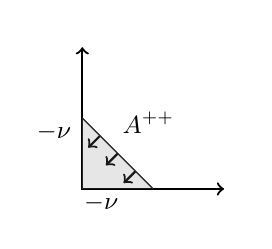
\begin{tikzpicture}[scale=0.6]
\draw [<->,thick] (0.0,3.0) node (yaxis) [above] {}
	|- (3.0,0.0) node (xaxis) [right] {};
\draw (0,1.5)  -- (1.5,0) ;
\draw [thick,->] (0.375,1.125) -- (0.125,0.875);
\draw [thick,->] (0.75,0.75) -- (0.5,0.5);
\draw [thick,->] (1.125,0.375) -- (0.875,0.125);
\node at (1.4,1.4) {\small $A^{++}$};
\node at (0.3999999999999999,-0.3) {\small $-\nu$};
\node at (-0.6,1.2) {\small $-\nu$};
\draw [fill=gray,opacity=0.2,gray] (1.5,0.0) -- (0.0,1.5) -- (0.0,0.0) ;
\end{tikzpicture}}
&{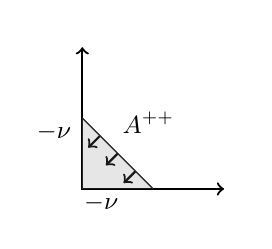
\begin{tikzpicture}[scale=0.6]
\draw [<->,thick] (0.0,3.0) node (yaxis) [above] {}
	|- (3.0,0.0) node (xaxis) [right] {};
\draw (0,1.5)  -- (1.5,0) ;
\draw [thick,->] (0.375,1.125) -- (0.125,0.875);
\draw [thick,->] (0.75,0.75) -- (0.5,0.5);
\draw [thick,->] (1.125,0.375) -- (0.875,0.125);
\node at (1.4,1.4) {\small $A^{++}$};
\node at (0.3999999999999999,-0.3) {\small $-\nu$};
\node at (-0.6,1.2) {\small $-\nu$};
\draw [fill=gray,opacity=0.2,gray] (1.5,0.0) -- (0.0,1.5) -- (0.0,0.0) ;
\end{tikzpicture}}
&{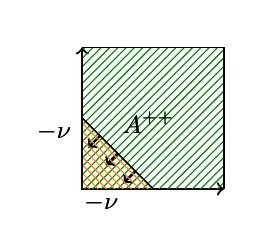
\begin{tikzpicture}[scale=0.6]
\draw [<->,thick] (0.0,3.0) node (yaxis) [above] {}
	|- (3.0,0.0) node (xaxis) [right] {};
\draw (0,1.5)  -- (1.5,0) ;
\draw [thick,->] (0.375,1.125) -- (0.125,0.875);
\draw [thick,->] (0.75,0.75) -- (0.5,0.5);
\draw [thick,->] (1.125,0.375) -- (0.875,0.125);
\node at (1.4,1.4) {\small $A^{++}$};
\node at (0.3999999999999999,-0.3) {\small $-\nu$};
\node at (-0.6,1.2) {\small $-\nu$};
\draw [pattern=north east lines, pattern color=green!50!black] (3.0,0.0) -- (3.0,3.0) -- (0.0,3.0) -- (0.0,0.0) ;
\draw (0,1.5)  -- (1.5,0) ;
\draw [thick,->] (0.375,1.125) -- (0.125,0.875);
\draw [thick,->] (0.75,0.75) -- (0.5,0.5);
\draw [thick,->] (1.125,0.375) -- (0.875,0.125);
\node at (1.4,1.4) {\small $A^{++}$};
\node at (0.3999999999999999,-0.3) {\small $-\nu$};
\node at (-0.6,1.2) {\small $-\nu$};
\draw [pattern=north west lines, pattern color=orange] (1.5,0.0) -- (0.0,1.5) -- (0.0,0.0) ;
\end{tikzpicture}}
\\[0pt]
      \vspace{-3cm}$\begin{array}{l}
	      \nu\todd\\ \nu\le\frac{n-3}{2}
      \end{array}$&{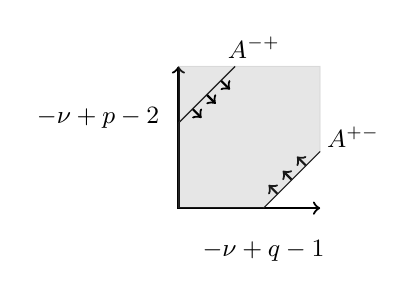
\begin{tikzpicture}[scale=0.6]
\draw [<->,thick] (0.0,3.0) node (yaxis) [above] {}
	|- (3.0,0.0) node (xaxis) [right] {};
\draw (1.8,0.0) -- (3.0,1.2) ;
\draw [thick,->] (2.1,0.3) -- (1.9100000000000001,0.49);
\draw [thick,->] (2.4,0.6) -- (2.21,0.79);
\draw [thick,->] (2.7,0.8999999999999999) -- (2.5100000000000002,1.0899999999999999);
\node at (3.7,1.5) {\small $A^{+-}$};
\node at (1.8,-0.9) {\small $-\nu+q-1$};
\draw [fill=gray,opacity=0.2,gray] (1.8,0.0) -- (3.0,1.2) -- (3.0,3.0) -- (1.2,3.0) -- (0.0,1.8) -- (0.0,0.0) ;
\draw (0.0,1.8) -- (1.2,3.0) ;
\draw [thick,->] (0.3,2.1) -- (0.49,1.9100000000000001);
\draw [thick,->] (0.6,2.4) -- (0.79,2.21);
\draw [thick,->] (0.8999999999999999,2.7) -- (1.0899999999999999,2.5100000000000002);
\node at (1.6,3.4) {\small $A^{-+}$};
\node at (-1.7,1.9000000000000001) {\small $-\nu+p-2$};
\draw [fill=gray,opacity=0.2,gray] (0.0,1.8) -- (1.2,3.0) -- (0.0,3.0) ;
\end{tikzpicture}}
&{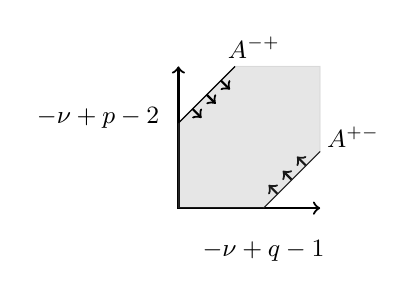
\begin{tikzpicture}[scale=0.6]
\draw [<->,thick] (0.0,3.0) node (yaxis) [above] {}
	|- (3.0,0.0) node (xaxis) [right] {};
\draw (1.8,0.0) -- (3.0,1.2) ;
\draw [thick,->] (2.1,0.3) -- (1.9100000000000001,0.49);
\draw [thick,->] (2.4,0.6) -- (2.21,0.79);
\draw [thick,->] (2.7,0.8999999999999999) -- (2.5100000000000002,1.0899999999999999);
\node at (3.7,1.5) {\small $A^{+-}$};
\node at (1.8,-0.9) {\small $-\nu+q-1$};
\draw [fill=gray,opacity=0.2,gray] (1.8,0.0) -- (3.0,1.2) -- (3.0,3.0) -- (1.2,3.0) -- (0.0,1.8) -- (0.0,0.0) ;
\draw (0.0,1.8) -- (1.2,3.0) ;
\draw [thick,->] (0.3,2.1) -- (0.49,1.9100000000000001);
\draw [thick,->] (0.6,2.4) -- (0.79,2.21);
\draw [thick,->] (0.8999999999999999,2.7) -- (1.0899999999999999,2.5100000000000002);
\node at (1.6,3.4) {\small $A^{-+}$};
\node at (-1.7,1.9000000000000001) {\small $-\nu+p-2$};
\end{tikzpicture}}
&{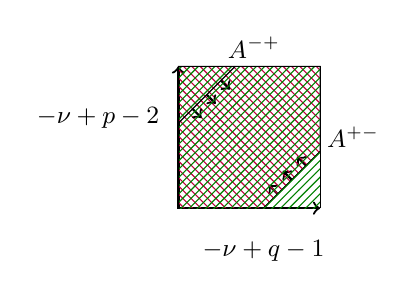
\begin{tikzpicture}[scale=0.6]
\draw [<->,thick] (0.0,3.0) node (yaxis) [above] {}
	|- (3.0,0.0) node (xaxis) [right] {};
\draw (1.8,0.0) -- (3.0,1.2) ;
\draw [thick,->] (2.1,0.3) -- (1.9100000000000001,0.49);
\draw [thick,->] (2.4,0.6) -- (2.21,0.79);
\draw [thick,->] (2.7,0.8999999999999999) -- (2.5100000000000002,1.0899999999999999);
\node at (3.7,1.5) {\small $A^{+-}$};
\node at (1.8,-0.9) {\small $-\nu+q-1$};
\draw [pattern=north west lines, pattern color=purple] (1.8,0.0) -- (3.0,1.2) -- (3.0,3.0) -- (0.0,3.0) -- (0.0,0.0) ;
\draw (0.0,1.8) -- (1.2,3.0) ;
\draw [thick,->] (0.3,2.1) -- (0.49,1.9100000000000001);
\draw [thick,->] (0.6,2.4) -- (0.79,2.21);
\draw [thick,->] (0.8999999999999999,2.7) -- (1.0899999999999999,2.5100000000000002);
\node at (1.6,3.4) {\small $A^{-+}$};
\node at (-1.7,1.9000000000000001) {\small $-\nu+p-2$};
\draw [pattern=north east lines, pattern color=green!50!black] (3.0,0.0) -- (3.0,3.0) -- (0.0,3.0) -- (0.0,0.0) ;
\end{tikzpicture}}
\\[0pt]
	      $(\lambda,\nu)\in$&$\mybra{//\cup\backslash\backslash}^c$ && $//\cap\backslash\backslash,k=l$\\[0pt]
	      \vspace{-3cm}$\begin{array}{l}\nu\todd\\\nu=\frac{n-1}{2}
	      \end{array}$&{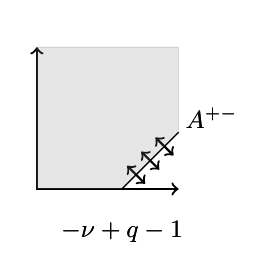
\begin{tikzpicture}[scale=0.6]
\draw [<->,thick] (0.0,3.0) node (yaxis) [above] {}
	|- (3.0,0.0) node (xaxis) [right] {};
\draw (1.8,0.0) -- (3.0,1.2) ;
\draw [thick,->] (2.1,0.3) -- (1.9100000000000001,0.49);
\draw [thick,->] (2.4,0.6) -- (2.21,0.79);
\draw [thick,->] (2.7,0.8999999999999999) -- (2.5100000000000002,1.0899999999999999);
\node at (3.7,1.5) {\small $A^{+-}$};
\node at (1.8,-0.9) {\small $-\nu+q-1$};
\draw [fill=gray,opacity=0.2,gray] (1.8,0.0) -- (3.0,1.2) -- (3.0,3.0) -- (0.0,3.0) -- (0.0,0.0) ;
\draw (1.8,0.0) -- (3.0,1.2) ;
\draw [thick,->] (2.1,0.3) -- (2.29,0.10999999999999999);
\draw [thick,->] (2.4,0.6) -- (2.59,0.41);
\draw [thick,->] (2.7,0.8999999999999999) -- (2.89,0.71);
\node at (3.7,1.5) {\small $A^{+-}$};
\node at (1.8,-0.9) {\small $-\nu+q-1$};
\end{tikzpicture}}
&&{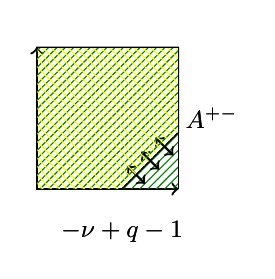
\begin{tikzpicture}[scale=0.6]
\draw [<->,thick] (0.0,3.0) node (yaxis) [above] {}
	|- (3.0,0.0) node (xaxis) [right] {};
\draw (1.8,0.0) -- (3.0,1.2) ;
\draw [thick,->] (2.1,0.3) -- (1.9100000000000001,0.49);
\draw [thick,->] (2.4,0.6) -- (2.21,0.79);
\draw [thick,->] (2.7,0.8999999999999999) -- (2.5100000000000002,1.0899999999999999);
\node at (3.7,1.5) {\small $A^{+-}$};
\node at (1.8,-0.9) {\small $-\nu+q-1$};
\draw [pattern=north east lines, pattern color=green!50!black] (3.0,0.0) -- (3.0,3.0) -- (0.0,3.0) -- (0.0,0.0) ;
\draw (1.8,0.0) -- (3.0,1.2) ;
\draw [thick,->] (2.1,0.3) -- (2.29,0.10999999999999999);
\draw [thick,->] (2.4,0.6) -- (2.59,0.41);
\draw [thick,->] (2.7,0.8999999999999999) -- (2.89,0.71);
\node at (3.7,1.5) {\small $A^{+-}$};
\node at (1.8,-0.9) {\small $-\nu+q-1$};
\draw [pattern=north west lines, pattern color=yellow] (1.8,0.0) -- (3.0,1.2) -- (3.0,3.0) -- (0.0,3.0) -- (0.0,0.0) ;
\end{tikzpicture}}
\\[0pt]
	      $(\lambda,\nu)\in$&$\mybra{//\cup\backslash\backslash}^c$ & $//-\backslash\backslash$  & $//\cap\backslash\backslash,k< l$\\[0pt]
	      \vspace{-3cm}$\begin{array}{l}\nu\teven\\\nu\ge{n-1}\end{array}$&{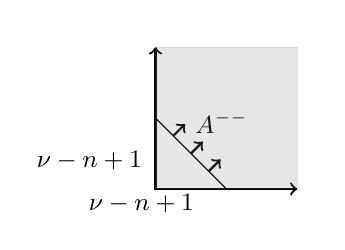
\begin{tikzpicture}[scale=0.6]
\draw [<->,thick] (0.0,3.0) node (yaxis) [above] {}
	|- (3.0,0.0) node (xaxis) [right] {};
\draw (0,1.5)  -- (1.5,0) ;
\draw [thick,->] (0.375,1.125) -- (0.625,1.375);
\draw [thick,->] (0.75,0.75) -- (1.0,1.0);
\draw [thick,->] (1.125,0.375) -- (1.375,0.625);
\node at (-1.4,0.6) {\small $\nu-n+1$};
\node at (-0.30000000000000004,-0.3) {\small $\nu-n+1$};
\node at (1.4,1.4) {\small $A^{--}$};
\draw [fill=gray,opacity=0.2,gray] (3.0,0.0) -- (3.0,3.0) -- (0.0,3.0) -- (0.0,0.0) ;
\end{tikzpicture}}\kern0.7cm
&{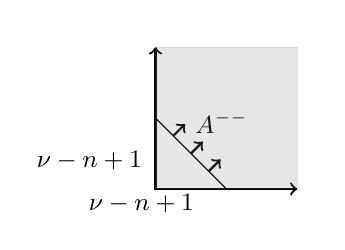
\begin{tikzpicture}[scale=0.6]
\draw [<->,thick] (0.0,3.0) node (yaxis) [above] {}
	|- (3.0,0.0) node (xaxis) [right] {};
\draw (0,1.5)  -- (1.5,0) ;
\draw [thick,->] (0.375,1.125) -- (0.625,1.375);
\draw [thick,->] (0.75,0.75) -- (1.0,1.0);
\draw [thick,->] (1.125,0.375) -- (1.375,0.625);
\node at (-1.4,0.6) {\small $\nu-n+1$};
\node at (-0.30000000000000004,-0.3) {\small $\nu-n+1$};
\node at (1.4,1.4) {\small $A^{--}$};
\draw [fill=gray,opacity=0.2,gray] (3.0,0.0) -- (3.0,3.0) -- (0.0,3.0) -- (0.0,0.0) ;
\end{tikzpicture}}\kern0.7cm
&{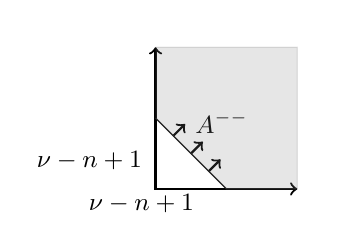
\begin{tikzpicture}[scale=0.6]
\draw [<->,thick] (0.0,3.0) node (yaxis) [above] {}
	|- (3.0,0.0) node (xaxis) [right] {};
\draw (0,1.5)  -- (1.5,0) ;
\draw [thick,->] (0.375,1.125) -- (0.625,1.375);
\draw [thick,->] (0.75,0.75) -- (1.0,1.0);
\draw [thick,->] (1.125,0.375) -- (1.375,0.625);
\node at (-1.4,0.6) {\small $\nu-n+1$};
\node at (-0.30000000000000004,-0.3) {\small $\nu-n+1$};
\node at (1.4,1.4) {\small $A^{--}$};
\draw [fill=gray,opacity=0.2,gray] (0.0,1.5) -- (1.5,0.0) -- (3.0,0.0) -- (3.0,3.0) -- (0.0,3.0) ;
\end{tikzpicture}}\kern0.7cm
\\[0pt]
	    \end{tabular}
	  \end{figure}
		\begin{figure}[H]
			\noindent\begin{tabular}{m{1.3cm}rrr}
	      $(\lambda,\nu)\in$&$\mybra{//\cup\backslash\backslash}^c$ & $//-\backslash\backslash$  & $//\cap\backslash\backslash,k< l$\\[0pt]
	      \vspace{-3cm}$\begin{array}{l}\nu\todd\\\nu\ge\frac{n+1}{2}\end{array}$&{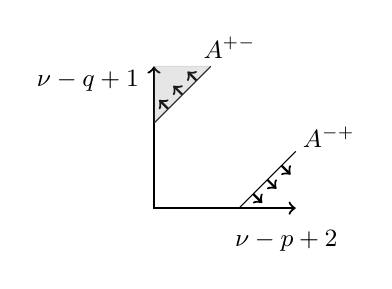
\begin{tikzpicture}[scale=0.6]
\draw [<->,thick] (0.0,3.0) node (yaxis) [above] {}
	|- (3.0,0.0) node (xaxis) [right] {};
\draw (1.8,0.0) -- (3.0,1.2) ;
\draw [thick,->] (2.1,0.3) -- (2.29,0.10999999999999999);
\draw [thick,->] (2.4,0.6) -- (2.59,0.41);
\draw [thick,->] (2.7,0.8999999999999999) -- (2.89,0.71);
\node at (3.7,1.5) {\small $A^{-+}$};
\node at (2.8,-0.7) {\small $\nu-p+2$};
\draw (0.0,1.8) -- (1.2,3.0) ;
\draw [thick,->] (0.3,2.1) -- (0.10999999999999999,2.29);
\draw [thick,->] (0.6,2.4) -- (0.41,2.59);
\draw [thick,->] (0.8999999999999999,2.7) -- (0.71,2.89);
\node at (1.6,3.4) {\small $A^{+-}$};
\node at (-1.4,2.7) {\small $\nu-q+1$};
\draw [fill=gray,opacity=0.2,gray] (0.0,1.8) -- (1.2,3.0) -- (0.0,3.0) ;
\end{tikzpicture}}
&{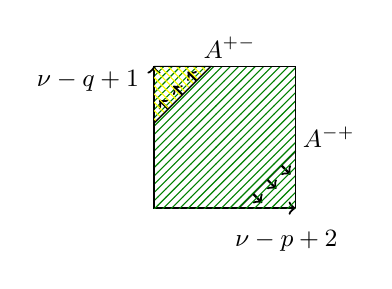
\begin{tikzpicture}[scale=0.6]
\draw [<->,thick] (0.0,3.0) node (yaxis) [above] {}
	|- (3.0,0.0) node (xaxis) [right] {};
\draw (1.8,0.0) -- (3.0,1.2) ;
\draw [thick,->] (2.1,0.3) -- (2.29,0.10999999999999999);
\draw [thick,->] (2.4,0.6) -- (2.59,0.41);
\draw [thick,->] (2.7,0.8999999999999999) -- (2.89,0.71);
\node at (3.7,1.5) {\small $A^{-+}$};
\node at (2.8,-0.7) {\small $\nu-p+2$};
\draw [pattern=north east lines, pattern color=green!50!black] (3.0,0.0) -- (3.0,3.0) -- (0.0,3.0) -- (0.0,0.0) ;
\draw (0.0,1.8) -- (1.2,3.0) ;
\draw [thick,->] (0.3,2.1) -- (0.10999999999999999,2.29);
\draw [thick,->] (0.6,2.4) -- (0.41,2.59);
\draw [thick,->] (0.8999999999999999,2.7) -- (0.71,2.89);
\node at (1.6,3.4) {\small $A^{+-}$};
\node at (-1.4,2.7) {\small $\nu-q+1$};
\draw [pattern=north west lines, pattern color=yellow] (0.0,1.8) -- (1.2,3.0) -- (0.0,3.0) ;
\end{tikzpicture}}
&{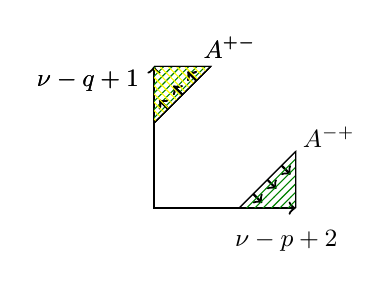
\begin{tikzpicture}[scale=0.6]
\draw [<->,thick] (0.0,3.0) node (yaxis) [above] {}
	|- (3.0,0.0) node (xaxis) [right] {};
\draw (1.8,0.0) -- (3.0,1.2) ;
\draw [thick,->] (2.1,0.3) -- (2.29,0.10999999999999999);
\draw [thick,->] (2.4,0.6) -- (2.59,0.41);
\draw [thick,->] (2.7,0.8999999999999999) -- (2.89,0.71);
\node at (3.7,1.5) {\small $A^{-+}$};
\node at (2.8,-0.7) {\small $\nu-p+2$};
\draw [pattern=north east lines, pattern color=green!50!black] (1.8,0.0) -- (3.0,1.2) -- (3.0,0.0) ;
\draw (0.0,1.8) -- (1.2,3.0) ;
\draw [thick,->] (0.3,2.1) -- (0.10999999999999999,2.29);
\draw [thick,->] (0.6,2.4) -- (0.41,2.59);
\draw [thick,->] (0.8999999999999999,2.7) -- (0.71,2.89);
\node at (1.6,3.4) {\small $A^{+-}$};
\node at (-1.4,2.7) {\small $\nu-q+1$};
\draw [pattern=north east lines, pattern color=green!50!black] (0.0,1.8) -- (1.2,3.0) -- (0.0,3.0) ;
\draw (0.0,1.8) -- (1.2,3.0) ;
\draw [thick,->] (0.3,2.1) -- (0.10999999999999999,2.29);
\draw [thick,->] (0.6,2.4) -- (0.41,2.59);
\draw [thick,->] (0.8999999999999999,2.7) -- (0.71,2.89);
\node at (1.6,3.4) {\small $A^{+-}$};
\node at (-1.4,2.7) {\small $\nu-q+1$};
\draw [pattern=north west lines, pattern color=yellow] (0.0,1.8) -- (1.2,3.0) -- (0.0,3.0) ;
\end{tikzpicture}}
\\[25pt]
	    \end{tabular}
	  \end{figure}
	\item Suppose $p,q\in\odd$ and $p>1$. Then,
		\begin{figure}[H]
			\noindent\begin{tabular}{m{1.3cm}rrr}
			$(\lambda,\nu)\in$&$\mybra{\ss\cup\bb}^c$ & $\bb-\ss$  & $\ss-\bb$\\[0pt]
			\tevenText{\le0}&{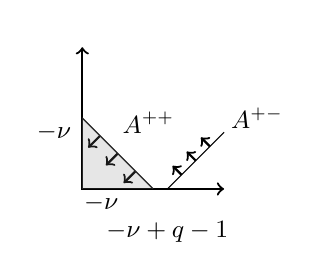
\begin{tikzpicture}[scale=0.6]
\draw [<->,thick] (0.0,3.0) node (yaxis) [above] {}
	|- (3.0,0.0) node (xaxis) [right] {};
\draw (0,1.5)  -- (1.5,0) ;
\draw [thick,->] (0.375,1.125) -- (0.125,0.875);
\draw [thick,->] (0.75,0.75) -- (0.5,0.5);
\draw [thick,->] (1.125,0.375) -- (0.875,0.125);
\node at (1.4,1.4) {\small $A^{++}$};
\node at (0.3999999999999999,-0.3) {\small $-\nu$};
\node at (-0.6,1.2) {\small $-\nu$};
\draw [fill=gray,opacity=0.2,gray] (1.5,0.0) -- (0.0,1.5) -- (0.0,0.0) ;
\draw (1.8,0.0) -- (3.0,1.2) ;
\draw [thick,->] (2.1,0.3) -- (1.9100000000000001,0.49);
\draw [thick,->] (2.4,0.6) -- (2.21,0.79);
\draw [thick,->] (2.7,0.8999999999999999) -- (2.5100000000000002,1.0899999999999999);
\node at (3.7,1.5) {\small $A^{+-}$};
\node at (1.8,-0.9) {\small $-\nu+q-1$};
\end{tikzpicture}}
&{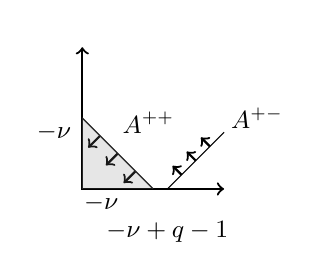
\begin{tikzpicture}[scale=0.6]
\draw [<->,thick] (0.0,3.0) node (yaxis) [above] {}
	|- (3.0,0.0) node (xaxis) [right] {};
\draw (0,1.5)  -- (1.5,0) ;
\draw [thick,->] (0.375,1.125) -- (0.125,0.875);
\draw [thick,->] (0.75,0.75) -- (0.5,0.5);
\draw [thick,->] (1.125,0.375) -- (0.875,0.125);
\node at (1.4,1.4) {\small $A^{++}$};
\node at (0.3999999999999999,-0.3) {\small $-\nu$};
\node at (-0.6,1.2) {\small $-\nu$};
\draw [fill=gray,opacity=0.2,gray] (1.5,0.0) -- (0.0,1.5) -- (0.0,0.0) ;
\draw (1.8,0.0) -- (3.0,1.2) ;
\draw [thick,->] (2.1,0.3) -- (1.9100000000000001,0.49);
\draw [thick,->] (2.4,0.6) -- (2.21,0.79);
\draw [thick,->] (2.7,0.8999999999999999) -- (2.5100000000000002,1.0899999999999999);
\node at (3.7,1.5) {\small $A^{+-}$};
\node at (1.8,-0.9) {\small $-\nu+q-1$};
\end{tikzpicture}}
&{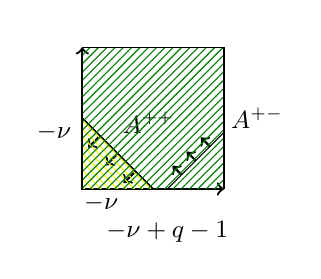
\begin{tikzpicture}[scale=0.6]
\draw [<->,thick] (0.0,3.0) node (yaxis) [above] {}
	|- (3.0,0.0) node (xaxis) [right] {};
\draw (0,1.5)  -- (1.5,0) ;
\draw [thick,->] (0.375,1.125) -- (0.125,0.875);
\draw [thick,->] (0.75,0.75) -- (0.5,0.5);
\draw [thick,->] (1.125,0.375) -- (0.875,0.125);
\node at (1.4,1.4) {\small $A^{++}$};
\node at (0.3999999999999999,-0.3) {\small $-\nu$};
\node at (-0.6,1.2) {\small $-\nu$};
\draw [pattern=north west lines, pattern color=yellow] (1.5,0.0) -- (0.0,1.5) -- (0.0,0.0) ;
\draw (1.8,0.0) -- (3.0,1.2) ;
\draw [thick,->] (2.1,0.3) -- (1.9100000000000001,0.49);
\draw [thick,->] (2.4,0.6) -- (2.21,0.79);
\draw [thick,->] (2.7,0.8999999999999999) -- (2.5100000000000002,1.0899999999999999);
\node at (3.7,1.5) {\small $A^{+-}$};
\node at (1.8,-0.9) {\small $-\nu+q-1$};
\draw [pattern=north east lines, pattern color=green!50!black] (3.0,0.0) -- (3.0,3.0) -- (0.0,3.0) -- (0.0,0.0) ;
\end{tikzpicture}}
\\[0pt]
			\toddText{\le n-3}&{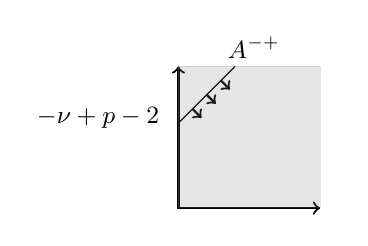
\begin{tikzpicture}[scale=0.6]
\draw [<->,thick] (0.0,3.0) node (yaxis) [above] {}
	|- (3.0,0.0) node (xaxis) [right] {};
\draw (0.0,1.8) -- (1.2,3.0) ;
\draw [thick,->] (0.3,2.1) -- (0.49,1.9100000000000001);
\draw [thick,->] (0.6,2.4) -- (0.79,2.21);
\draw [thick,->] (0.8999999999999999,2.7) -- (1.0899999999999999,2.5100000000000002);
\node at (1.6,3.4) {\small $A^{-+}$};
\node at (-1.7,1.9000000000000001) {\small $-\nu+p-2$};
\draw [fill=gray,opacity=0.2,gray] (3.0,0.0) -- (3.0,3.0) -- (0.0,3.0) -- (0.0,0.0) ;
\end{tikzpicture}}
&{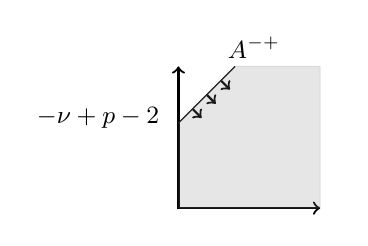
\begin{tikzpicture}[scale=0.6]
\draw [<->,thick] (0.0,3.0) node (yaxis) [above] {}
	|- (3.0,0.0) node (xaxis) [right] {};
\draw (0.0,1.8) -- (1.2,3.0) ;
\draw [thick,->] (0.3,2.1) -- (0.49,1.9100000000000001);
\draw [thick,->] (0.6,2.4) -- (0.79,2.21);
\draw [thick,->] (0.8999999999999999,2.7) -- (1.0899999999999999,2.5100000000000002);
\node at (1.6,3.4) {\small $A^{-+}$};
\node at (-1.7,1.9000000000000001) {\small $-\nu+p-2$};
\draw [fill=gray,opacity=0.2,gray] (0.0,1.8) -- (1.2,3.0) -- (3.0,3.0) -- (3.0,0.0) -- (0.0,0.0) ;
\end{tikzpicture}}
&{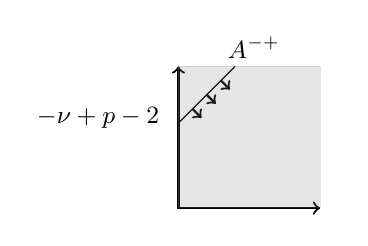
\begin{tikzpicture}[scale=0.6]
\draw [<->,thick] (0.0,3.0) node (yaxis) [above] {}
	|- (3.0,0.0) node (xaxis) [right] {};
\draw (0.0,1.8) -- (1.2,3.0) ;
\draw [thick,->] (0.3,2.1) -- (0.49,1.9100000000000001);
\draw [thick,->] (0.6,2.4) -- (0.79,2.21);
\draw [thick,->] (0.8999999999999999,2.7) -- (1.0899999999999999,2.5100000000000002);
\node at (1.6,3.4) {\small $A^{-+}$};
\node at (-1.7,1.9000000000000001) {\small $-\nu+p-2$};
\draw [fill=gray,opacity=0.2,gray] (3.0,0.0) -- (3.0,3.0) -- (0.0,3.0) -- (0.0,0.0) ;
\end{tikzpicture}}
\\[0pt]
			\tevenText{>0}&{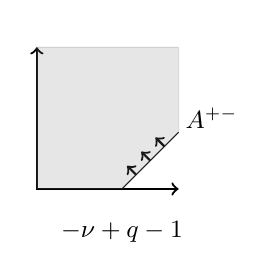
\begin{tikzpicture}[scale=0.6]
\draw [<->,thick] (0.0,3.0) node (yaxis) [above] {}
	|- (3.0,0.0) node (xaxis) [right] {};
\draw (1.8,0.0) -- (3.0,1.2) ;
\draw [thick,->] (2.1,0.3) -- (1.9100000000000001,0.49);
\draw [thick,->] (2.4,0.6) -- (2.21,0.79);
\draw [thick,->] (2.7,0.8999999999999999) -- (2.5100000000000002,1.0899999999999999);
\node at (3.7,1.5) {\small $A^{+-}$};
\node at (1.8,-0.9) {\small $-\nu+q-1$};
\draw [fill=gray,opacity=0.2,gray] (1.8,0.0) -- (3.0,1.2) -- (3.0,3.0) -- (0.0,3.0) -- (0.0,0.0) ;
\end{tikzpicture}}
&{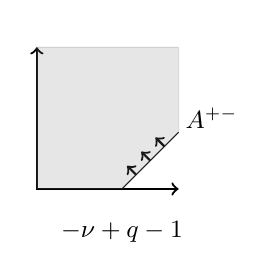
\begin{tikzpicture}[scale=0.6]
\draw [<->,thick] (0.0,3.0) node (yaxis) [above] {}
	|- (3.0,0.0) node (xaxis) [right] {};
\draw (1.8,0.0) -- (3.0,1.2) ;
\draw [thick,->] (2.1,0.3) -- (1.9100000000000001,0.49);
\draw [thick,->] (2.4,0.6) -- (2.21,0.79);
\draw [thick,->] (2.7,0.8999999999999999) -- (2.5100000000000002,1.0899999999999999);
\node at (3.7,1.5) {\small $A^{+-}$};
\node at (1.8,-0.9) {\small $-\nu+q-1$};
\draw [fill=gray,opacity=0.2,gray] (1.8,0.0) -- (3.0,1.2) -- (3.0,3.0) -- (0.0,3.0) -- (0.0,0.0) ;
\end{tikzpicture}}
&{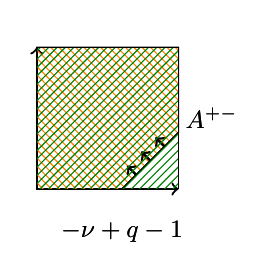
\begin{tikzpicture}[scale=0.6]
\draw [<->,thick] (0.0,3.0) node (yaxis) [above] {}
	|- (3.0,0.0) node (xaxis) [right] {};
\draw (1.8,0.0) -- (3.0,1.2) ;
\draw [thick,->] (2.1,0.3) -- (1.9100000000000001,0.49);
\draw [thick,->] (2.4,0.6) -- (2.21,0.79);
\draw [thick,->] (2.7,0.8999999999999999) -- (2.5100000000000002,1.0899999999999999);
\node at (3.7,1.5) {\small $A^{+-}$};
\node at (1.8,-0.9) {\small $-\nu+q-1$};
\draw [pattern=north west lines, pattern color=orange] (1.8,0.0) -- (3.0,1.2) -- (3.0,3.0) -- (0.0,3.0) -- (0.0,0.0) ;
\draw (1.8,0.0) -- (3.0,1.2) ;
\draw [thick,->] (2.1,0.3) -- (1.9100000000000001,0.49);
\draw [thick,->] (2.4,0.6) -- (2.21,0.79);
\draw [thick,->] (2.7,0.8999999999999999) -- (2.5100000000000002,1.0899999999999999);
\node at (3.7,1.5) {\small $A^{+-}$};
\node at (1.8,-0.9) {\small $-\nu+q-1$};
\draw [pattern=north east lines, pattern color=green!50!black] (3.0,0.0) -- (3.0,3.0) -- (0.0,3.0) -- (0.0,0.0) ;
\end{tikzpicture}}
\\[0pt]
			\toddText{>n-3}&{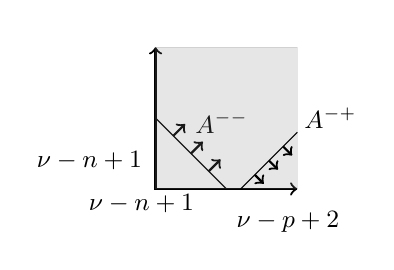
\begin{tikzpicture}[scale=0.6]
\draw [<->,thick] (0.0,3.0) node (yaxis) [above] {}
	|- (3.0,0.0) node (xaxis) [right] {};
\draw (0,1.5)  -- (1.5,0) ;
\draw [thick,->] (0.375,1.125) -- (0.625,1.375);
\draw [thick,->] (0.75,0.75) -- (1.0,1.0);
\draw [thick,->] (1.125,0.375) -- (1.375,0.625);
\node at (-1.4,0.6) {\small $\nu-n+1$};
\node at (-0.30000000000000004,-0.3) {\small $\nu-n+1$};
\node at (1.4,1.4) {\small $A^{--}$};
\draw [fill=gray,opacity=0.2,gray] (3.0,0.0) -- (3.0,3.0) -- (0.0,3.0) -- (0.0,0.0) ;
\draw (1.8,0.0) -- (3.0,1.2) ;
\draw [thick,->] (2.1,0.3) -- (2.29,0.10999999999999999);
\draw [thick,->] (2.4,0.6) -- (2.59,0.41);
\draw [thick,->] (2.7,0.8999999999999999) -- (2.89,0.71);
\node at (3.7,1.5) {\small $A^{-+}$};
\node at (2.8,-0.7) {\small $\nu-p+2$};
\end{tikzpicture}\kern-0.7cm}
&{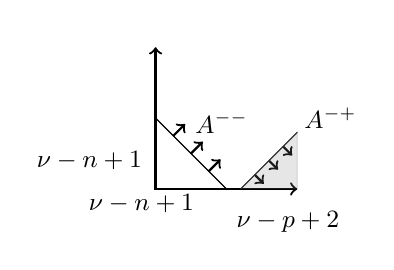
\begin{tikzpicture}[scale=0.6]
\draw [<->,thick] (0.0,3.0) node (yaxis) [above] {}
	|- (3.0,0.0) node (xaxis) [right] {};
\draw (0,1.5)  -- (1.5,0) ;
\draw [thick,->] (0.375,1.125) -- (0.625,1.375);
\draw [thick,->] (0.75,0.75) -- (1.0,1.0);
\draw [thick,->] (1.125,0.375) -- (1.375,0.625);
\node at (-1.4,0.6) {\small $\nu-n+1$};
\node at (-0.30000000000000004,-0.3) {\small $\nu-n+1$};
\node at (1.4,1.4) {\small $A^{--}$};
\draw (1.8,0.0) -- (3.0,1.2) ;
\draw [thick,->] (2.1,0.3) -- (2.29,0.10999999999999999);
\draw [thick,->] (2.4,0.6) -- (2.59,0.41);
\draw [thick,->] (2.7,0.8999999999999999) -- (2.89,0.71);
\node at (3.7,1.5) {\small $A^{-+}$};
\node at (2.8,-0.7) {\small $\nu-p+2$};
\draw [fill=gray,opacity=0.2,gray] (1.8,0.0) -- (3.0,1.2) -- (3.0,0.0) ;
\end{tikzpicture}\kern-0.7cm}
&{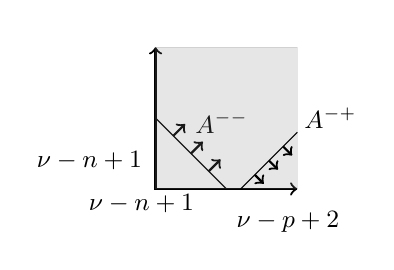
\begin{tikzpicture}[scale=0.6]
\draw [<->,thick] (0.0,3.0) node (yaxis) [above] {}
	|- (3.0,0.0) node (xaxis) [right] {};
\draw (0,1.5)  -- (1.5,0) ;
\draw [thick,->] (0.375,1.125) -- (0.625,1.375);
\draw [thick,->] (0.75,0.75) -- (1.0,1.0);
\draw [thick,->] (1.125,0.375) -- (1.375,0.625);
\node at (-1.4,0.6) {\small $\nu-n+1$};
\node at (-0.30000000000000004,-0.3) {\small $\nu-n+1$};
\node at (1.4,1.4) {\small $A^{--}$};
\draw [fill=gray,opacity=0.2,gray] (3.0,0.0) -- (3.0,3.0) -- (0.0,3.0) -- (0.0,0.0) ;
\draw (1.8,0.0) -- (3.0,1.2) ;
\draw [thick,->] (2.1,0.3) -- (2.29,0.10999999999999999);
\draw [thick,->] (2.4,0.6) -- (2.59,0.41);
\draw [thick,->] (2.7,0.8999999999999999) -- (2.89,0.71);
\node at (3.7,1.5) {\small $A^{-+}$};
\node at (2.8,-0.7) {\small $\nu-p+2$};
\end{tikzpicture}\kern-0.7cm}
\\[0pt]
			  
		\end{tabular}
		\end{figure}
	\item Suppose $p,q\in\even$. Then,
		\begin{figure}[H]
			\noindent\begin{tabular}{m{1.3cm}rrr}
			$(\lambda,\nu)\in$&$\mybra{\ss\cup\bb}^c$ & $\bb-\ss$  & $\ss-\bb$\\[0pt]
			\tevenText{\le0}&{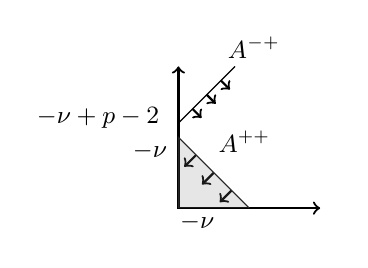
\begin{tikzpicture}[scale=0.6]
\draw [<->,thick] (0.0,3.0) node (yaxis) [above] {}
	|- (3.0,0.0) node (xaxis) [right] {};
\draw (0,1.5)  -- (1.5,0) ;
\draw [thick,->] (0.375,1.125) -- (0.125,0.875);
\draw [thick,->] (0.75,0.75) -- (0.5,0.5);
\draw [thick,->] (1.125,0.375) -- (0.875,0.125);
\node at (1.4,1.4) {\small $A^{++}$};
\node at (0.3999999999999999,-0.3) {\small $-\nu$};
\node at (-0.6,1.2) {\small $-\nu$};
\draw [fill=gray,opacity=0.2,gray] (1.5,0.0) -- (0.0,1.5) -- (0.0,0.0) ;
\draw (0.0,1.8) -- (1.2,3.0) ;
\draw [thick,->] (0.3,2.1) -- (0.49,1.9100000000000001);
\draw [thick,->] (0.6,2.4) -- (0.79,2.21);
\draw [thick,->] (0.8999999999999999,2.7) -- (1.0899999999999999,2.5100000000000002);
\node at (1.6,3.4) {\small $A^{-+}$};
\node at (-1.7,1.9000000000000001) {\small $-\nu+p-2$};
\end{tikzpicture}}
&{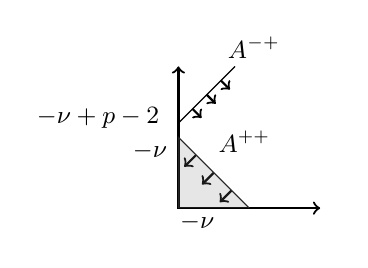
\begin{tikzpicture}[scale=0.6]
\draw [<->,thick] (0.0,3.0) node (yaxis) [above] {}
	|- (3.0,0.0) node (xaxis) [right] {};
\draw (0,1.5)  -- (1.5,0) ;
\draw [thick,->] (0.375,1.125) -- (0.125,0.875);
\draw [thick,->] (0.75,0.75) -- (0.5,0.5);
\draw [thick,->] (1.125,0.375) -- (0.875,0.125);
\node at (1.4,1.4) {\small $A^{++}$};
\node at (0.3999999999999999,-0.3) {\small $-\nu$};
\node at (-0.6,1.2) {\small $-\nu$};
\draw [fill=gray,opacity=0.2,gray] (1.5,0.0) -- (0.0,1.5) -- (0.0,0.0) ;
\draw (0.0,1.8) -- (1.2,3.0) ;
\draw [thick,->] (0.3,2.1) -- (0.49,1.9100000000000001);
\draw [thick,->] (0.6,2.4) -- (0.79,2.21);
\draw [thick,->] (0.8999999999999999,2.7) -- (1.0899999999999999,2.5100000000000002);
\node at (1.6,3.4) {\small $A^{-+}$};
\node at (-1.7,1.9000000000000001) {\small $-\nu+p-2$};
\end{tikzpicture}}
&{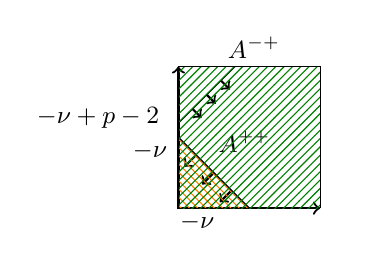
\begin{tikzpicture}[scale=0.6]
\draw [<->,thick] (0.0,3.0) node (yaxis) [above] {}
	|- (3.0,0.0) node (xaxis) [right] {};
\draw (0,1.5)  -- (1.5,0) ;
\draw [thick,->] (0.375,1.125) -- (0.125,0.875);
\draw [thick,->] (0.75,0.75) -- (0.5,0.5);
\draw [thick,->] (1.125,0.375) -- (0.875,0.125);
\node at (1.4,1.4) {\small $A^{++}$};
\node at (0.3999999999999999,-0.3) {\small $-\nu$};
\node at (-0.6,1.2) {\small $-\nu$};
\draw [pattern=north west lines, pattern color=orange] (1.5,0.0) -- (0.0,1.5) -- (0.0,0.0) ;
\draw (0.0,1.8) -- (1.2,3.0) ;
\draw [thick,->] (0.3,2.1) -- (0.49,1.9100000000000001);
\draw [thick,->] (0.6,2.4) -- (0.79,2.21);
\draw [thick,->] (0.8999999999999999,2.7) -- (1.0899999999999999,2.5100000000000002);
\node at (1.6,3.4) {\small $A^{-+}$};
\node at (-1.7,1.9000000000000001) {\small $-\nu+p-2$};
\draw [pattern=north east lines, pattern color=green!50!black] (3.0,0.0) -- (3.0,3.0) -- (0.0,3.0) -- (0.0,0.0) ;
\end{tikzpicture}}
\\[0pt]
			\toddText{\le n-3}&{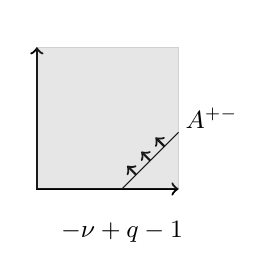
\begin{tikzpicture}[scale=0.6]
\draw [<->,thick] (0.0,3.0) node (yaxis) [above] {}
	|- (3.0,0.0) node (xaxis) [right] {};
\draw (1.8,0.0) -- (3.0,1.2) ;
\draw [thick,->] (2.1,0.3) -- (1.9100000000000001,0.49);
\draw [thick,->] (2.4,0.6) -- (2.21,0.79);
\draw [thick,->] (2.7,0.8999999999999999) -- (2.5100000000000002,1.0899999999999999);
\node at (3.7,1.5) {\small $A^{+-}$};
\node at (1.8,-0.9) {\small $-\nu+q-1$};
\draw [fill=gray,opacity=0.2,gray] (3.0,0.0) -- (3.0,3.0) -- (0.0,3.0) -- (0.0,0.0) ;
\end{tikzpicture}}
&{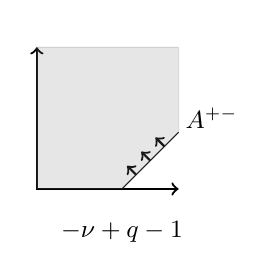
\begin{tikzpicture}[scale=0.6]
\draw [<->,thick] (0.0,3.0) node (yaxis) [above] {}
	|- (3.0,0.0) node (xaxis) [right] {};
\draw (1.8,0.0) -- (3.0,1.2) ;
\draw [thick,->] (2.1,0.3) -- (1.9100000000000001,0.49);
\draw [thick,->] (2.4,0.6) -- (2.21,0.79);
\draw [thick,->] (2.7,0.8999999999999999) -- (2.5100000000000002,1.0899999999999999);
\node at (3.7,1.5) {\small $A^{+-}$};
\node at (1.8,-0.9) {\small $-\nu+q-1$};
\draw [fill=gray,opacity=0.2,gray] (1.8,0.0) -- (3.0,1.2) -- (3.0,3.0) -- (0.0,3.0) -- (0.0,0.0) ;
\end{tikzpicture}}
&{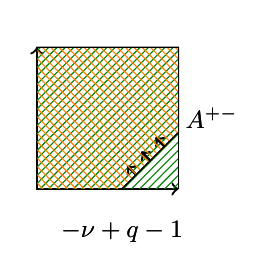
\begin{tikzpicture}[scale=0.6]
\draw [<->,thick] (0.0,3.0) node (yaxis) [above] {}
	|- (3.0,0.0) node (xaxis) [right] {};
\draw (1.8,0.0) -- (3.0,1.2) ;
\draw [thick,->] (2.1,0.3) -- (1.9100000000000001,0.49);
\draw [thick,->] (2.4,0.6) -- (2.21,0.79);
\draw [thick,->] (2.7,0.8999999999999999) -- (2.5100000000000002,1.0899999999999999);
\node at (3.7,1.5) {\small $A^{+-}$};
\node at (1.8,-0.9) {\small $-\nu+q-1$};
\draw [pattern=north east lines, pattern color=green!50!black] (3.0,0.0) -- (3.0,3.0) -- (0.0,3.0) -- (0.0,0.0) ;
\draw (1.8,0.0) -- (3.0,1.2) ;
\draw [thick,->] (2.1,0.3) -- (1.9100000000000001,0.49);
\draw [thick,->] (2.4,0.6) -- (2.21,0.79);
\draw [thick,->] (2.7,0.8999999999999999) -- (2.5100000000000002,1.0899999999999999);
\node at (3.7,1.5) {\small $A^{+-}$};
\node at (1.8,-0.9) {\small $-\nu+q-1$};
\draw [pattern=north west lines, pattern color=orange] (1.8,0.0) -- (3.0,1.2) -- (3.0,3.0) -- (0.0,3.0) -- (0.0,0.0) ;
\end{tikzpicture}}
\\[0pt]
			\tevenText{>0}&{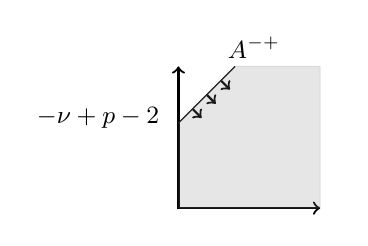
\begin{tikzpicture}[scale=0.6]
\draw [<->,thick] (0.0,3.0) node (yaxis) [above] {}
	|- (3.0,0.0) node (xaxis) [right] {};
\draw (0.0,1.8) -- (1.2,3.0) ;
\draw [thick,->] (0.3,2.1) -- (0.49,1.9100000000000001);
\draw [thick,->] (0.6,2.4) -- (0.79,2.21);
\draw [thick,->] (0.8999999999999999,2.7) -- (1.0899999999999999,2.5100000000000002);
\node at (1.6,3.4) {\small $A^{-+}$};
\node at (-1.7,1.9000000000000001) {\small $-\nu+p-2$};
\draw [fill=gray,opacity=0.2,gray] (0.0,1.8) -- (1.2,3.0) -- (3.0,3.0) -- (3.0,0.0) -- (0.0,0.0) ;
\end{tikzpicture}}
&{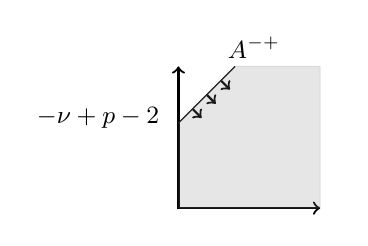
\begin{tikzpicture}[scale=0.6]
\draw [<->,thick] (0.0,3.0) node (yaxis) [above] {}
	|- (3.0,0.0) node (xaxis) [right] {};
\draw (0.0,1.8) -- (1.2,3.0) ;
\draw [thick,->] (0.3,2.1) -- (0.49,1.9100000000000001);
\draw [thick,->] (0.6,2.4) -- (0.79,2.21);
\draw [thick,->] (0.8999999999999999,2.7) -- (1.0899999999999999,2.5100000000000002);
\node at (1.6,3.4) {\small $A^{-+}$};
\node at (-1.7,1.9000000000000001) {\small $-\nu+p-2$};
\draw [fill=gray,opacity=0.2,gray] (0.0,1.8) -- (1.2,3.0) -- (3.0,3.0) -- (3.0,0.0) -- (0.0,0.0) ;
\end{tikzpicture}}
&{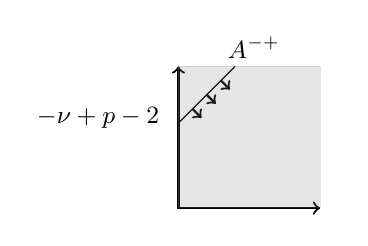
\begin{tikzpicture}[scale=0.6]
\draw [<->,thick] (0.0,3.0) node (yaxis) [above] {}
	|- (3.0,0.0) node (xaxis) [right] {};
\draw (0.0,1.8) -- (1.2,3.0) ;
\draw [thick,->] (0.3,2.1) -- (0.49,1.9100000000000001);
\draw [thick,->] (0.6,2.4) -- (0.79,2.21);
\draw [thick,->] (0.8999999999999999,2.7) -- (1.0899999999999999,2.5100000000000002);
\node at (1.6,3.4) {\small $A^{-+}$};
\node at (-1.7,1.9000000000000001) {\small $-\nu+p-2$};
\draw [fill=gray,opacity=0.2,gray] (3.0,0.0) -- (3.0,3.0) -- (0.0,3.0) -- (0.0,0.0) ;
\end{tikzpicture}}
\\[0pt]
			\toddText{>n-3}&{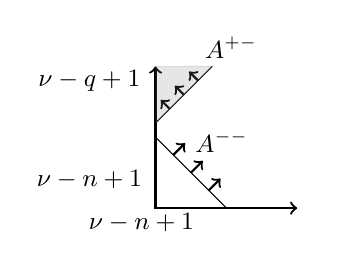
\begin{tikzpicture}[scale=0.6]
\draw [<->,thick] (0.0,3.0) node (yaxis) [above] {}
	|- (3.0,0.0) node (xaxis) [right] {};
\draw (0,1.5)  -- (1.5,0) ;
\draw [thick,->] (0.375,1.125) -- (0.625,1.375);
\draw [thick,->] (0.75,0.75) -- (1.0,1.0);
\draw [thick,->] (1.125,0.375) -- (1.375,0.625);
\node at (-1.4,0.6) {\small $\nu-n+1$};
\node at (-0.30000000000000004,-0.3) {\small $\nu-n+1$};
\node at (1.4,1.4) {\small $A^{--}$};
\draw (0.0,1.8) -- (1.2,3.0) ;
\draw [thick,->] (0.3,2.1) -- (0.10999999999999999,2.29);
\draw [thick,->] (0.6,2.4) -- (0.41,2.59);
\draw [thick,->] (0.8999999999999999,2.7) -- (0.71,2.89);
\node at (1.6,3.4) {\small $A^{+-}$};
\node at (-1.4,2.7) {\small $\nu-q+1$};
\draw [fill=gray,opacity=0.2,gray] (0.0,1.8) -- (1.2,3.0) -- (0.0,3.0) ;
\end{tikzpicture}}
&{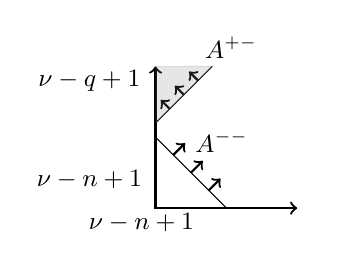
\begin{tikzpicture}[scale=0.6]
\draw [<->,thick] (0.0,3.0) node (yaxis) [above] {}
	|- (3.0,0.0) node (xaxis) [right] {};
\draw (0,1.5)  -- (1.5,0) ;
\draw [thick,->] (0.375,1.125) -- (0.625,1.375);
\draw [thick,->] (0.75,0.75) -- (1.0,1.0);
\draw [thick,->] (1.125,0.375) -- (1.375,0.625);
\node at (-1.4,0.6) {\small $\nu-n+1$};
\node at (-0.30000000000000004,-0.3) {\small $\nu-n+1$};
\node at (1.4,1.4) {\small $A^{--}$};
\draw (0.0,1.8) -- (1.2,3.0) ;
\draw [thick,->] (0.3,2.1) -- (0.10999999999999999,2.29);
\draw [thick,->] (0.6,2.4) -- (0.41,2.59);
\draw [thick,->] (0.8999999999999999,2.7) -- (0.71,2.89);
\node at (1.6,3.4) {\small $A^{+-}$};
\node at (-1.4,2.7) {\small $\nu-q+1$};
\draw [fill=gray,opacity=0.2,gray] (0.0,1.8) -- (1.2,3.0) -- (0.0,3.0) ;
\end{tikzpicture}}
&{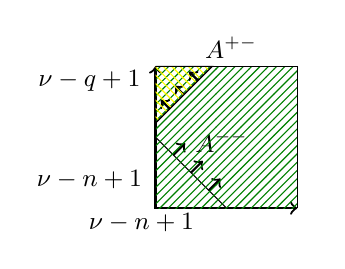
\begin{tikzpicture}[scale=0.6]
\draw [<->,thick] (0.0,3.0) node (yaxis) [above] {}
	|- (3.0,0.0) node (xaxis) [right] {};
\draw (0,1.5)  -- (1.5,0) ;
\draw [thick,->] (0.375,1.125) -- (0.625,1.375);
\draw [thick,->] (0.75,0.75) -- (1.0,1.0);
\draw [thick,->] (1.125,0.375) -- (1.375,0.625);
\node at (-1.4,0.6) {\small $\nu-n+1$};
\node at (-0.30000000000000004,-0.3) {\small $\nu-n+1$};
\node at (1.4,1.4) {\small $A^{--}$};
\draw [pattern=north east lines, pattern color=green!50!black] (3.0,0.0) -- (3.0,3.0) -- (0.0,3.0) -- (0.0,0.0) ;
\draw (0.0,1.8) -- (1.2,3.0) ;
\draw [thick,->] (0.3,2.1) -- (0.10999999999999999,2.29);
\draw [thick,->] (0.6,2.4) -- (0.41,2.59);
\draw [thick,->] (0.8999999999999999,2.7) -- (0.71,2.89);
\node at (1.6,3.4) {\small $A^{+-}$};
\node at (-1.4,2.7) {\small $\nu-q+1$};
\draw [pattern=north west lines, pattern color=yellow] (0.0,1.8) -- (1.2,3.0) -- (0.0,3.0) ;
\end{tikzpicture}}
\\[0pt]
		\end{tabular}
		\end{figure}
	\item Suppose $p\in\even,q\in\odd$. Then for $\nu\in\odd$, $R_{\lambda,\nu}^X$ is surjective. Otherwise (for $\nu\in\even$) we have,
	  \begin{figure}[H]
		  \noindent\begin{tabular}{@{}m{1.6cm}@{}ccc}
	      $(\lambda,\nu)\in$&$\mybra{//\cup\backslash\backslash}^c$ & $\backslash\backslash-//$  & $//\cap\backslash\backslash,k> l$\\[0pt]
	      \vspace{-3cm}$\nu\leq0$&{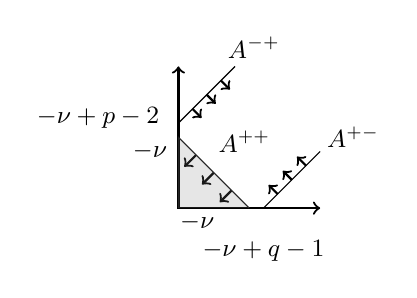
\begin{tikzpicture}[scale=0.6]
\draw [<->,thick] (0.0,3.0) node (yaxis) [above] {}
	|- (3.0,0.0) node (xaxis) [right] {};
\draw (0,1.5)  -- (1.5,0) ;
\draw [thick,->] (0.375,1.125) -- (0.125,0.875);
\draw [thick,->] (0.75,0.75) -- (0.5,0.5);
\draw [thick,->] (1.125,0.375) -- (0.875,0.125);
\node at (1.4,1.4) {\small $A^{++}$};
\node at (0.3999999999999999,-0.3) {\small $-\nu$};
\node at (-0.6,1.2) {\small $-\nu$};
\draw [fill=gray,opacity=0.2,gray] (1.5,0.0) -- (0.0,1.5) -- (0.0,0.0) ;
\draw (1.8,0.0) -- (3.0,1.2) ;
\draw [thick,->] (2.1,0.3) -- (1.9100000000000001,0.49);
\draw [thick,->] (2.4,0.6) -- (2.21,0.79);
\draw [thick,->] (2.7,0.8999999999999999) -- (2.5100000000000002,1.0899999999999999);
\node at (3.7,1.5) {\small $A^{+-}$};
\node at (1.8,-0.9) {\small $-\nu+q-1$};
\draw (0.0,1.8) -- (1.2,3.0) ;
\draw [thick,->] (0.3,2.1) -- (0.49,1.9100000000000001);
\draw [thick,->] (0.6,2.4) -- (0.79,2.21);
\draw [thick,->] (0.8999999999999999,2.7) -- (1.0899999999999999,2.5100000000000002);
\node at (1.6,3.4) {\small $A^{-+}$};
\node at (-1.7,1.9000000000000001) {\small $-\nu+p-2$};
\end{tikzpicture}}
&{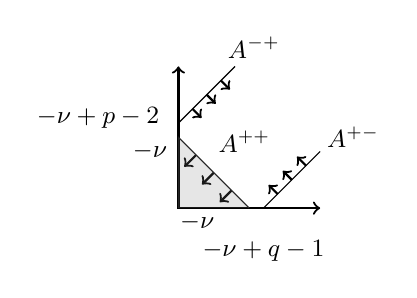
\begin{tikzpicture}[scale=0.6]
\draw [<->,thick] (0.0,3.0) node (yaxis) [above] {}
	|- (3.0,0.0) node (xaxis) [right] {};
\draw (0,1.5)  -- (1.5,0) ;
\draw [thick,->] (0.375,1.125) -- (0.125,0.875);
\draw [thick,->] (0.75,0.75) -- (0.5,0.5);
\draw [thick,->] (1.125,0.375) -- (0.875,0.125);
\node at (1.4,1.4) {\small $A^{++}$};
\node at (0.3999999999999999,-0.3) {\small $-\nu$};
\node at (-0.6,1.2) {\small $-\nu$};
\draw [fill=gray,opacity=0.2,gray] (1.5,0.0) -- (0.0,1.5) -- (0.0,0.0) ;
\draw (1.8,0.0) -- (3.0,1.2) ;
\draw [thick,->] (2.1,0.3) -- (1.9100000000000001,0.49);
\draw [thick,->] (2.4,0.6) -- (2.21,0.79);
\draw [thick,->] (2.7,0.8999999999999999) -- (2.5100000000000002,1.0899999999999999);
\node at (3.7,1.5) {\small $A^{+-}$};
\node at (1.8,-0.9) {\small $-\nu+q-1$};
\draw (0.0,1.8) -- (1.2,3.0) ;
\draw [thick,->] (0.3,2.1) -- (0.49,1.9100000000000001);
\draw [thick,->] (0.6,2.4) -- (0.79,2.21);
\draw [thick,->] (0.8999999999999999,2.7) -- (1.0899999999999999,2.5100000000000002);
\node at (1.6,3.4) {\small $A^{-+}$};
\node at (-1.7,1.9000000000000001) {\small $-\nu+p-2$};
\end{tikzpicture}}
&{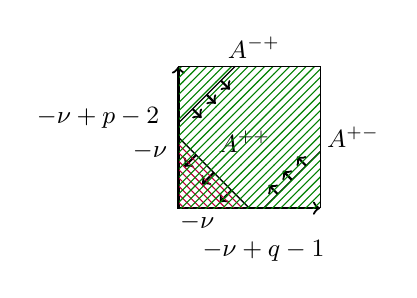
\begin{tikzpicture}[scale=0.6]
\draw [<->,thick] (0.0,3.0) node (yaxis) [above] {}
	|- (3.0,0.0) node (xaxis) [right] {};
\draw (0,1.5)  -- (1.5,0) ;
\draw [thick,->] (0.375,1.125) -- (0.125,0.875);
\draw [thick,->] (0.75,0.75) -- (0.5,0.5);
\draw [thick,->] (1.125,0.375) -- (0.875,0.125);
\node at (1.4,1.4) {\small $A^{++}$};
\node at (0.3999999999999999,-0.3) {\small $-\nu$};
\node at (-0.6,1.2) {\small $-\nu$};
\draw [pattern=north west lines, pattern color=purple] (1.5,0.0) -- (0.0,1.5) -- (0.0,0.0) ;
\draw (1.8,0.0) -- (3.0,1.2) ;
\draw [thick,->] (2.1,0.3) -- (1.9100000000000001,0.49);
\draw [thick,->] (2.4,0.6) -- (2.21,0.79);
\draw [thick,->] (2.7,0.8999999999999999) -- (2.5100000000000002,1.0899999999999999);
\node at (3.7,1.5) {\small $A^{+-}$};
\node at (1.8,-0.9) {\small $-\nu+q-1$};
\draw [pattern=north east lines, pattern color=green!50!black] (3.0,0.0) -- (3.0,3.0) -- (0.0,3.0) -- (0.0,0.0) ;
\draw (0.0,1.8) -- (1.2,3.0) ;
\draw [thick,->] (0.3,2.1) -- (0.49,1.9100000000000001);
\draw [thick,->] (0.6,2.4) -- (0.79,2.21);
\draw [thick,->] (0.8999999999999999,2.7) -- (1.0899999999999999,2.5100000000000002);
\node at (1.6,3.4) {\small $A^{-+}$};
\node at (-1.7,1.9000000000000001) {\small $-\nu+p-2$};
\end{tikzpicture}}
\\[0pt]
	      \vspace{-3cm}$
	      \begin{array}{l}
		      \nu>0\\\nu\le\frac{n-3}{2}
	      \end{array}
	      $&{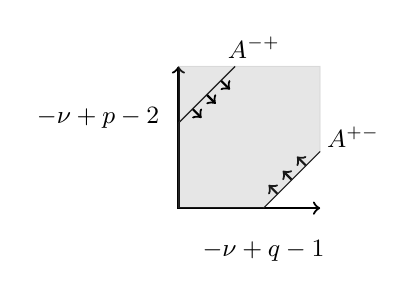
\begin{tikzpicture}[scale=0.6]
\draw [<->,thick] (0.0,3.0) node (yaxis) [above] {}
	|- (3.0,0.0) node (xaxis) [right] {};
\draw (1.8,0.0) -- (3.0,1.2) ;
\draw [thick,->] (2.1,0.3) -- (1.9100000000000001,0.49);
\draw [thick,->] (2.4,0.6) -- (2.21,0.79);
\draw [thick,->] (2.7,0.8999999999999999) -- (2.5100000000000002,1.0899999999999999);
\node at (3.7,1.5) {\small $A^{+-}$};
\node at (1.8,-0.9) {\small $-\nu+q-1$};
\draw [fill=gray,opacity=0.2,gray] (1.8,0.0) -- (3.0,1.2) -- (3.0,3.0) -- (1.2,3.0) -- (0.0,1.8) -- (0.0,0.0) ;
\draw (0.0,1.8) -- (1.2,3.0) ;
\draw [thick,->] (0.3,2.1) -- (0.49,1.9100000000000001);
\draw [thick,->] (0.6,2.4) -- (0.79,2.21);
\draw [thick,->] (0.8999999999999999,2.7) -- (1.0899999999999999,2.5100000000000002);
\node at (1.6,3.4) {\small $A^{-+}$};
\node at (-1.7,1.9000000000000001) {\small $-\nu+p-2$};
\draw [fill=gray,opacity=0.2,gray] (0.0,1.8) -- (1.2,3.0) -- (0.0,3.0) ;
\end{tikzpicture}}
&{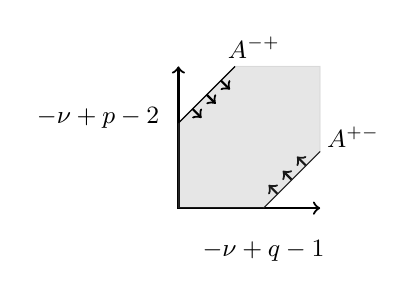
\begin{tikzpicture}[scale=0.6]
\draw [<->,thick] (0.0,3.0) node (yaxis) [above] {}
	|- (3.0,0.0) node (xaxis) [right] {};
\draw (1.8,0.0) -- (3.0,1.2) ;
\draw [thick,->] (2.1,0.3) -- (1.9100000000000001,0.49);
\draw [thick,->] (2.4,0.6) -- (2.21,0.79);
\draw [thick,->] (2.7,0.8999999999999999) -- (2.5100000000000002,1.0899999999999999);
\node at (3.7,1.5) {\small $A^{+-}$};
\node at (1.8,-0.9) {\small $-\nu+q-1$};
\draw [fill=gray,opacity=0.2,gray] (1.8,0.0) -- (3.0,1.2) -- (3.0,3.0) -- (1.2,3.0) -- (0.0,1.8) -- (0.0,0.0) ;
\draw (0.0,1.8) -- (1.2,3.0) ;
\draw [thick,->] (0.3,2.1) -- (0.49,1.9100000000000001);
\draw [thick,->] (0.6,2.4) -- (0.79,2.21);
\draw [thick,->] (0.8999999999999999,2.7) -- (1.0899999999999999,2.5100000000000002);
\node at (1.6,3.4) {\small $A^{-+}$};
\node at (-1.7,1.9000000000000001) {\small $-\nu+p-2$};
\end{tikzpicture}}
&{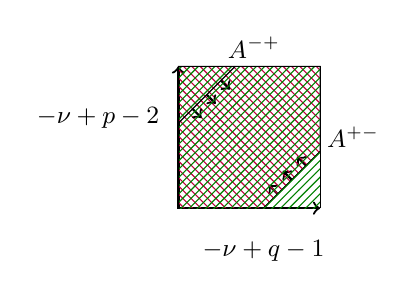
\begin{tikzpicture}[scale=0.6]
\draw [<->,thick] (0.0,3.0) node (yaxis) [above] {}
	|- (3.0,0.0) node (xaxis) [right] {};
\draw (1.8,0.0) -- (3.0,1.2) ;
\draw [thick,->] (2.1,0.3) -- (1.9100000000000001,0.49);
\draw [thick,->] (2.4,0.6) -- (2.21,0.79);
\draw [thick,->] (2.7,0.8999999999999999) -- (2.5100000000000002,1.0899999999999999);
\node at (3.7,1.5) {\small $A^{+-}$};
\node at (1.8,-0.9) {\small $-\nu+q-1$};
\draw [pattern=north west lines, pattern color=purple] (1.8,0.0) -- (3.0,1.2) -- (3.0,3.0) -- (0.0,3.0) -- (0.0,0.0) ;
\draw (0.0,1.8) -- (1.2,3.0) ;
\draw [thick,->] (0.3,2.1) -- (0.49,1.9100000000000001);
\draw [thick,->] (0.6,2.4) -- (0.79,2.21);
\draw [thick,->] (0.8999999999999999,2.7) -- (1.0899999999999999,2.5100000000000002);
\node at (1.6,3.4) {\small $A^{-+}$};
\node at (-1.7,1.9000000000000001) {\small $-\nu+p-2$};
\draw [pattern=north east lines, pattern color=green!50!black] (3.0,0.0) -- (3.0,3.0) -- (0.0,3.0) -- (0.0,0.0) ;
\end{tikzpicture}}
\\[0pt]
              $(\lambda,\nu)\in$&$\mybra{//\cup\backslash\backslash}^c$ && $//\cap\backslash\backslash,k=l$\\[0pt]
	      \vspace{-3cm}$
	      \begin{array}{l}
		      \nu\todd\\\nu=\frac{n-1}{2}
	      \end{array}
	      $&{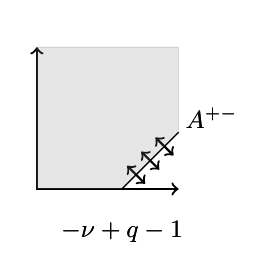
\begin{tikzpicture}[scale=0.6]
\draw [<->,thick] (0.0,3.0) node (yaxis) [above] {}
	|- (3.0,0.0) node (xaxis) [right] {};
\draw (1.8,0.0) -- (3.0,1.2) ;
\draw [thick,->] (2.1,0.3) -- (1.9100000000000001,0.49);
\draw [thick,->] (2.4,0.6) -- (2.21,0.79);
\draw [thick,->] (2.7,0.8999999999999999) -- (2.5100000000000002,1.0899999999999999);
\node at (3.7,1.5) {\small $A^{+-}$};
\node at (1.8,-0.9) {\small $-\nu+q-1$};
\draw [fill=gray,opacity=0.2,gray] (1.8,0.0) -- (3.0,1.2) -- (3.0,3.0) -- (0.0,3.0) -- (0.0,0.0) ;
\draw (1.8,0.0) -- (3.0,1.2) ;
\draw [thick,->] (2.1,0.3) -- (2.29,0.10999999999999999);
\draw [thick,->] (2.4,0.6) -- (2.59,0.41);
\draw [thick,->] (2.7,0.8999999999999999) -- (2.89,0.71);
\node at (3.7,1.5) {\small $A^{+-}$};
\node at (1.8,-0.9) {\small $-\nu+q-1$};
\end{tikzpicture}}
&&{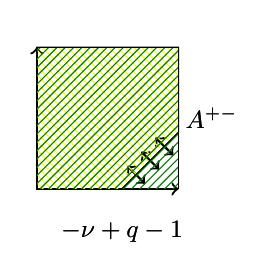
\begin{tikzpicture}[scale=0.6]
\draw [<->,thick] (0.0,3.0) node (yaxis) [above] {}
	|- (3.0,0.0) node (xaxis) [right] {};
\draw (1.8,0.0) -- (3.0,1.2) ;
\draw [thick,->] (2.1,0.3) -- (1.9100000000000001,0.49);
\draw [thick,->] (2.4,0.6) -- (2.21,0.79);
\draw [thick,->] (2.7,0.8999999999999999) -- (2.5100000000000002,1.0899999999999999);
\node at (3.7,1.5) {\small $A^{+-}$};
\node at (1.8,-0.9) {\small $-\nu+q-1$};
\draw [pattern=north west lines, pattern color=yellow] (1.8,0.0) -- (3.0,1.2) -- (3.0,3.0) -- (0.0,3.0) -- (0.0,0.0) ;
\draw (1.8,0.0) -- (3.0,1.2) ;
\draw [thick,->] (2.1,0.3) -- (2.29,0.10999999999999999);
\draw [thick,->] (2.4,0.6) -- (2.59,0.41);
\draw [thick,->] (2.7,0.8999999999999999) -- (2.89,0.71);
\node at (3.7,1.5) {\small $A^{+-}$};
\node at (1.8,-0.9) {\small $-\nu+q-1$};
\draw [pattern=north east lines, pattern color=green!50!black] (3.0,0.0) -- (3.0,3.0) -- (0.0,3.0) -- (0.0,0.0) ;
\end{tikzpicture}}
\\[0pt]
	      $(\lambda,\nu)\in$&$\mybra{//\cup\backslash\backslash}^c$ & $//-\backslash\backslash$  & $//\cap\backslash\backslash,k< l$\\[0pt]
	      \vspace{-3cm}
	      $
	      \begin{array}{l}
		      \nu\ge\frac{n+1}{2}\\\nu\le n-3
	      \end{array}
	      $
	      &{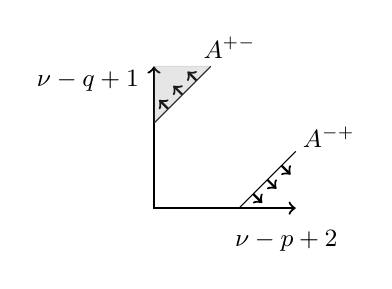
\begin{tikzpicture}[scale=0.6]
\draw [<->,thick] (0.0,3.0) node (yaxis) [above] {}
	|- (3.0,0.0) node (xaxis) [right] {};
\draw (1.8,0.0) -- (3.0,1.2) ;
\draw [thick,->] (2.1,0.3) -- (2.29,0.10999999999999999);
\draw [thick,->] (2.4,0.6) -- (2.59,0.41);
\draw [thick,->] (2.7,0.8999999999999999) -- (2.89,0.71);
\node at (3.7,1.5) {\small $A^{-+}$};
\node at (2.8,-0.7) {\small $\nu-p+2$};
\draw (0.0,1.8) -- (1.2,3.0) ;
\draw [thick,->] (0.3,2.1) -- (0.10999999999999999,2.29);
\draw [thick,->] (0.6,2.4) -- (0.41,2.59);
\draw [thick,->] (0.8999999999999999,2.7) -- (0.71,2.89);
\node at (1.6,3.4) {\small $A^{+-}$};
\node at (-1.4,2.7) {\small $\nu-q+1$};
\draw [fill=gray,opacity=0.2,gray] (0.0,1.8) -- (1.2,3.0) -- (0.0,3.0) ;
\end{tikzpicture}}
&{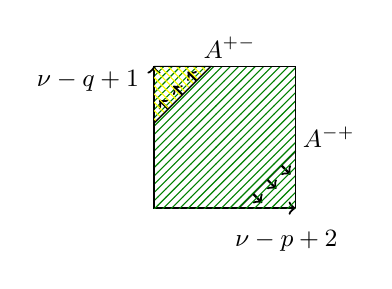
\begin{tikzpicture}[scale=0.6]
\draw [<->,thick] (0.0,3.0) node (yaxis) [above] {}
	|- (3.0,0.0) node (xaxis) [right] {};
\draw (1.8,0.0) -- (3.0,1.2) ;
\draw [thick,->] (2.1,0.3) -- (2.29,0.10999999999999999);
\draw [thick,->] (2.4,0.6) -- (2.59,0.41);
\draw [thick,->] (2.7,0.8999999999999999) -- (2.89,0.71);
\node at (3.7,1.5) {\small $A^{-+}$};
\node at (2.8,-0.7) {\small $\nu-p+2$};
\draw [pattern=north east lines, pattern color=green!50!black] (3.0,0.0) -- (3.0,3.0) -- (0.0,3.0) -- (0.0,0.0) ;
\draw (0.0,1.8) -- (1.2,3.0) ;
\draw [thick,->] (0.3,2.1) -- (0.10999999999999999,2.29);
\draw [thick,->] (0.6,2.4) -- (0.41,2.59);
\draw [thick,->] (0.8999999999999999,2.7) -- (0.71,2.89);
\node at (1.6,3.4) {\small $A^{+-}$};
\node at (-1.4,2.7) {\small $\nu-q+1$};
\draw [pattern=north west lines, pattern color=yellow] (0.0,1.8) -- (1.2,3.0) -- (0.0,3.0) ;
\end{tikzpicture}}
&{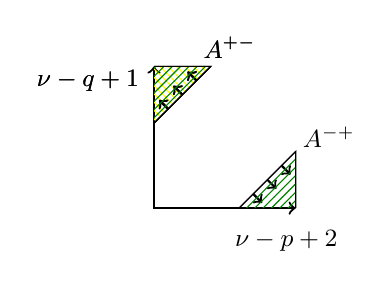
\begin{tikzpicture}[scale=0.6]
\draw [<->,thick] (0.0,3.0) node (yaxis) [above] {}
	|- (3.0,0.0) node (xaxis) [right] {};
\draw (1.8,0.0) -- (3.0,1.2) ;
\draw [thick,->] (2.1,0.3) -- (2.29,0.10999999999999999);
\draw [thick,->] (2.4,0.6) -- (2.59,0.41);
\draw [thick,->] (2.7,0.8999999999999999) -- (2.89,0.71);
\node at (3.7,1.5) {\small $A^{-+}$};
\node at (2.8,-0.7) {\small $\nu-p+2$};
\draw [pattern=north east lines, pattern color=green!50!black] (1.8,0.0) -- (3.0,1.2) -- (3.0,0.0) ;
\draw (0.0,1.8) -- (1.2,3.0) ;
\draw [thick,->] (0.3,2.1) -- (0.10999999999999999,2.29);
\draw [thick,->] (0.6,2.4) -- (0.41,2.59);
\draw [thick,->] (0.8999999999999999,2.7) -- (0.71,2.89);
\node at (1.6,3.4) {\small $A^{+-}$};
\node at (-1.4,2.7) {\small $\nu-q+1$};
\draw [pattern=north west lines, pattern color=yellow] (0.0,1.8) -- (1.2,3.0) -- (0.0,3.0) ;
\draw (0.0,1.8) -- (1.2,3.0) ;
\draw [thick,->] (0.3,2.1) -- (0.10999999999999999,2.29);
\draw [thick,->] (0.6,2.4) -- (0.41,2.59);
\draw [thick,->] (0.8999999999999999,2.7) -- (0.71,2.89);
\node at (1.6,3.4) {\small $A^{+-}$};
\node at (-1.4,2.7) {\small $\nu-q+1$};
\draw [pattern=north east lines, pattern color=green!50!black] (0.0,1.8) -- (1.2,3.0) -- (0.0,3.0) ;
\end{tikzpicture}}
\\[0pt]
	      \vspace{-3cm}$
	      \nu>n-3$&{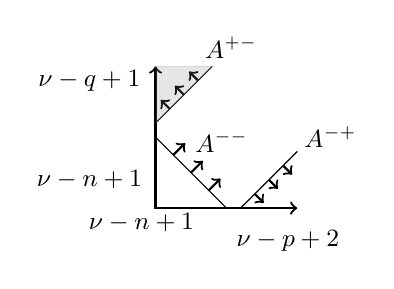
\begin{tikzpicture}[scale=0.6]
\draw [<->,thick] (0.0,3.0) node (yaxis) [above] {}
	|- (3.0,0.0) node (xaxis) [right] {};
\draw (0,1.5)  -- (1.5,0) ;
\draw [thick,->] (0.375,1.125) -- (0.625,1.375);
\draw [thick,->] (0.75,0.75) -- (1.0,1.0);
\draw [thick,->] (1.125,0.375) -- (1.375,0.625);
\node at (-1.4,0.6) {\small $\nu-n+1$};
\node at (-0.30000000000000004,-0.3) {\small $\nu-n+1$};
\node at (1.4,1.4) {\small $A^{--}$};
\draw (1.8,0.0) -- (3.0,1.2) ;
\draw [thick,->] (2.1,0.3) -- (2.29,0.10999999999999999);
\draw [thick,->] (2.4,0.6) -- (2.59,0.41);
\draw [thick,->] (2.7,0.8999999999999999) -- (2.89,0.71);
\node at (3.7,1.5) {\small $A^{-+}$};
\node at (2.8,-0.7) {\small $\nu-p+2$};
\draw (0.0,1.8) -- (1.2,3.0) ;
\draw [thick,->] (0.3,2.1) -- (0.10999999999999999,2.29);
\draw [thick,->] (0.6,2.4) -- (0.41,2.59);
\draw [thick,->] (0.8999999999999999,2.7) -- (0.71,2.89);
\node at (1.6,3.4) {\small $A^{+-}$};
\node at (-1.4,2.7) {\small $\nu-q+1$};
\draw [fill=gray,opacity=0.2,gray] (0.0,1.8) -- (1.2,3.0) -- (0.0,3.0) ;
\end{tikzpicture}}
&{\begin{tikzpicture}[scale=0.6]
\draw [<->,thick] (0.0,3.0) node (yaxis) [above] {}
	|- (3.0,0.0) node (xaxis) [right] {};
\draw (0,1.5)  -- (1.5,0) ;
\draw [thick,->] (0.375,1.125) -- (0.625,1.375);
\draw [thick,->] (0.75,0.75) -- (1.0,1.0);
\draw [thick,->] (1.125,0.375) -- (1.375,0.625);
\node at (-1.4,0.6) {\small $\nu-n+1$};
\node at (-0.30000000000000004,-0.3) {\small $\nu-n+1$};
\node at (1.4,1.4) {\small $A^{--}$};
\draw (1.8,0.0) -- (3.0,1.2) ;
\draw [thick,->] (2.1,0.3) -- (2.29,0.10999999999999999);
\draw [thick,->] (2.4,0.6) -- (2.59,0.41);
\draw [thick,->] (2.7,0.8999999999999999) -- (2.89,0.71);
\node at (3.7,1.5) {\small $A^{-+}$};
\node at (2.8,-0.7) {\small $\nu-p+2$};
\draw [pattern=north east lines, pattern color=green!50!black] (3.0,0.0) -- (3.0,3.0) -- (0.0,3.0) -- (0.0,0.0) ;
\draw (0.0,1.8) -- (1.2,3.0) ;
\draw [thick,->] (0.3,2.1) -- (0.10999999999999999,2.29);
\draw [thick,->] (0.6,2.4) -- (0.41,2.59);
\draw [thick,->] (0.8999999999999999,2.7) -- (0.71,2.89);
\node at (1.6,3.4) {\small $A^{+-}$};
\node at (-1.4,2.7) {\small $\nu-q+1$};
\draw [pattern=north west lines, pattern color=orange] (0.0,1.8) -- (1.2,3.0) -- (0.0,3.0) ;
\end{tikzpicture}}
&{\begin{tikzpicture}[scale=0.6]
\draw [<->,thick] (0.0,3.0) node (yaxis) [above] {}
	|- (3.0,0.0) node (xaxis) [right] {};
\draw (0,1.5)  -- (1.5,0) ;
\draw [thick,->] (0.375,1.125) -- (0.625,1.375);
\draw [thick,->] (0.75,0.75) -- (1.0,1.0);
\draw [thick,->] (1.125,0.375) -- (1.375,0.625);
\node at (-1.4,0.6) {\small $\nu-n+1$};
\node at (-0.30000000000000004,-0.3) {\small $\nu-n+1$};
\node at (1.4,1.4) {\small $A^{--}$};
\draw (1.8,0.0) -- (3.0,1.2) ;
\draw [thick,->] (2.1,0.3) -- (2.29,0.10999999999999999);
\draw [thick,->] (2.4,0.6) -- (2.59,0.41);
\draw [thick,->] (2.7,0.8999999999999999) -- (2.89,0.71);
\node at (3.7,1.5) {\small $A^{-+}$};
\node at (2.8,-0.7) {\small $\nu-p+2$};
\draw [pattern=north east lines, pattern color=green!50!black] (1.8,0.0) -- (3.0,1.2) -- (3.0,0.0) ;
\draw (0.0,1.8) -- (1.2,3.0) ;
\draw [thick,->] (0.3,2.1) -- (0.10999999999999999,2.29);
\draw [thick,->] (0.6,2.4) -- (0.41,2.59);
\draw [thick,->] (0.8999999999999999,2.7) -- (0.71,2.89);
\node at (1.6,3.4) {\small $A^{+-}$};
\node at (-1.4,2.7) {\small $\nu-q+1$};
\draw [pattern=north west lines, pattern color=orange] (0.0,1.8) -- (1.2,3.0) -- (0.0,3.0) ;
\draw (0.0,1.8) -- (1.2,3.0) ;
\draw [thick,->] (0.3,2.1) -- (0.10999999999999999,2.29);
\draw [thick,->] (0.6,2.4) -- (0.41,2.59);
\draw [thick,->] (0.8999999999999999,2.7) -- (0.71,2.89);
\node at (1.6,3.4) {\small $A^{+-}$};
\node at (-1.4,2.7) {\small $\nu-q+1$};
\draw [pattern=north east lines, pattern color=green!50!black] (0.0,1.8) -- (1.2,3.0) -- (0.0,3.0) ;
\end{tikzpicture}}
\\[0pt]
	    \end{tabular}
	  \end{figure}
	\end{enumerate}
	\vspace{-0.9cm}
	In the diagrams above some of them are filled not with gray, but with colored diagonal lines. This means that the image of the regular
	SBO $R_{\lambda,\nu}^X$ is zero and the (green/purple)
	ascending/descending diagonal lines show the images of its residues $R_{\lambda,\nu}^{ \left\{ o \right\}}$ and $\tilde{R}_{\lambda,\nu}^X$ respectively.

	For $p=1$ we have:\\
	\newcommand{\mystack}[2]{$\begin{array}{l}#1\\#2\end{array}$}
	\begin{figure}[H]
		\begin{tabular}{p{3.2cm}p{2.0cm}p{2.0cm}p{2.0cm}p{2.3cm}p{2.3cm}}
		$(\lambda,\nu)\in$ & $\mybra{\ss\cup\bb}^c$ & $\ss-\bb$ & $\bb-\ss$ & $\ss\cap\bb,k<l$ & $\ss\cap\bb,k\geq l$\\
		\vspace{-0.7cm}\mystack{\nu\teven}{\nu\le0}&{\begin{tikzpicture}[scale=0.6]
\draw[thick] (0.0,0.0)  -- (3.0,0.0) ;
\draw[fill=black] (0.0,0.0) circle (2pt);
\draw[fill=black] (1.5,0.0) circle (2pt);
\node at (1.5,0) {\huge ]};
\node[align=center, above] at (1.5,0.5) {\small $-\nu$}
;\draw [fill=gray,opacity=0.2,gray] (-0.05,-0.36) -- (-0.05,0.36) -- (1.55,0.36) -- (1.55,-0.36) 
;\end{tikzpicture}}
&{\begin{tikzpicture}[scale=0.6]
\draw[thick] (0.0,0.0)  -- (3.0,0.0) ;
\draw[fill=black] (0.0,0.0) circle (2pt);
\draw[fill=black] (1.5,0.0) circle (2pt);
\node at (1.5,0) {\huge ]};
\node[align=center, above] at (1.5,0.5) {\small $-\nu$}
;\draw [pattern=north west lines, pattern color=orange] (-0.05,-0.36) -- (-0.05,0.36) -- (1.55,0.36) -- (1.55,-0.36) 
;\draw[fill=black] (1.5,0.0) circle (2pt);
\node at (1.5,0) {\huge ]};
\node[align=center, above] at (1.5,0.5) {\small $-\nu$}
;\draw [pattern=north east lines, pattern color=green!50!black] (-0.05,-0.36) -- (-0.05,0.36) -- (3.05,0.36) -- (3.05,-0.36) 
;\end{tikzpicture}}
&{\begin{tikzpicture}[scale=0.6]
\draw[thick] (0.0,0.0)  -- (3.0,0.0) ;
\draw[fill=black] (0.0,0.0) circle (2pt);
\draw[fill=black] (1.5,0.0) circle (2pt);
\node at (1.5,0) {\huge ]};
\node[align=center, above] at (1.5,0.5) {\small $-\nu$}
;\draw [fill=gray,opacity=0.2,gray] (-0.05,-0.36) -- (-0.05,0.36) -- (1.55,0.36) -- (1.55,-0.36) 
;\end{tikzpicture}}
&{\vspace{-0.7cm}$\quad\;\;\quad\times$}&{\begin{tikzpicture}[scale=0.6]
\draw[thick] (0.0,0.0)  -- (3.0,0.0) ;
\draw[fill=black] (0.0,0.0) circle (2pt);
\draw[fill=black] (1.5,0.0) circle (2pt);
\node at (1.5,0) {\huge ]};
\node[align=center, above] at (1.5,0.5) {\small $-\nu$}
;\draw [pattern=north east lines, pattern color=green!50!black] (-0.05,-0.36) -- (-0.05,0.36) -- (3.05,0.36) -- (3.05,-0.36) 
;\draw[fill=black] (1.5,0.0) circle (2pt);
\node at (1.5,0) {\huge ]};
\node[align=center, above] at (1.5,0.5) {\small $-\nu$}
;\draw [pattern=north west lines, pattern color=orange] (-0.05,-0.36) -- (-0.05,0.36) -- (1.55,0.36) -- (1.55,-0.36) 
;\end{tikzpicture}}
\\
		\vspace{-0.5cm}\mystack{\nu,q\teven}{0<\nu<q}&{\begin{tikzpicture}[scale=0.6]
\draw[thick] (0.0,0.0)  -- (3.0,0.0) ;
\draw[fill=black] (0.0,0.0) circle (2pt);
\draw [fill=gray,opacity=0.2,gray] (-0.05,-0.36) -- (-0.05,0.36) -- (3.05,0.36) -- (3.05,-0.36) 
;\end{tikzpicture}}
&{\begin{tikzpicture}[scale=0.6]
\draw[thick] (0.0,0.0)  -- (3.0,0.0) ;
\draw[fill=black] (0.0,0.0) circle (2pt);
\draw [fill=gray,opacity=0.2,gray] (-0.05,-0.36) -- (-0.05,0.36) -- (3.05,0.36) -- (3.05,-0.36) 
;\end{tikzpicture}}
&{\begin{tikzpicture}[scale=0.6]
\draw[thick] (0.0,0.0)  -- (3.0,0.0) ;
\draw[fill=black] (0.0,0.0) circle (2pt);
\draw [fill=gray,opacity=0.2,gray] (-0.05,-0.36) -- (-0.05,0.36) -- (3.05,0.36) -- (3.05,-0.36) 
;\end{tikzpicture}}
&{\begin{tikzpicture}[scale=0.6]
\draw[thick] (0.0,0.0)  -- (3.0,0.0) ;
\draw[fill=black] (0.0,0.0) circle (2pt);
\draw [fill=gray,opacity=0.2,gray] (-0.05,-0.36) -- (-0.05,0.36) -- (3.05,0.36) -- (3.05,-0.36) 
;\end{tikzpicture}}
&{\begin{tikzpicture}[scale=0.6]
\draw[thick] (0.0,0.0)  -- (3.0,0.0) ;
\draw[fill=black] (0.0,0.0) circle (2pt);
\draw [fill=gray,opacity=0.2,gray] (-0.05,-0.36) -- (-0.05,0.36) -- (3.05,0.36) -- (3.05,-0.36) 
;\end{tikzpicture}}
\\
		\vspace{-0.5cm}\mystack{\nu\teven,q\todd}{0<\nu<q}&{\begin{tikzpicture}[scale=0.6]
\draw[thick] (0.0,0.0)  -- (3.0,0.0) ;
\draw[fill=black] (0.0,0.0) circle (2pt);
\draw [fill=gray,opacity=0.2,gray] (-0.05,-0.36) -- (-0.05,0.36) -- (3.05,0.36) -- (3.05,-0.36) 
;\end{tikzpicture}}
&{\begin{tikzpicture}[scale=0.6]
\draw[thick] (0.0,0.0)  -- (3.0,0.0) ;
\draw[fill=black] (0.0,0.0) circle (2pt);
\draw [pattern=north west lines, pattern color=yellow] (-0.05,-0.36) -- (-0.05,0.36) -- (3.05,0.36) -- (3.05,-0.36) 
;\draw [pattern=north east lines, pattern color=green!50!black] (-0.05,-0.36) -- (-0.05,0.36) -- (3.05,0.36) -- (3.05,-0.36) 
;\end{tikzpicture}}
&{\begin{tikzpicture}[scale=0.6]
\draw[thick] (0.0,0.0)  -- (3.0,0.0) ;
\draw[fill=black] (0.0,0.0) circle (2pt);
\draw [fill=gray,opacity=0.2,gray] (-0.05,-0.36) -- (-0.05,0.36) -- (3.05,0.36) -- (3.05,-0.36) 
;\end{tikzpicture}}
&{\begin{tikzpicture}[scale=0.6]
\draw[thick] (0.0,0.0)  -- (3.0,0.0) ;
\draw[fill=black] (0.0,0.0) circle (2pt);
\draw [fill=gray,opacity=0.2,gray] (-0.05,-0.36) -- (-0.05,0.36) -- (3.05,0.36) -- (3.05,-0.36) 
;\end{tikzpicture}}
&{\begin{tikzpicture}[scale=0.6]
\draw[thick] (0.0,0.0)  -- (3.0,0.0) ;
\draw[fill=black] (0.0,0.0) circle (2pt);
\draw [fill=gray,opacity=0.2,gray] (-0.05,-0.36) -- (-0.05,0.36) -- (3.05,0.36) -- (3.05,-0.36) 
;\end{tikzpicture}}
\\
		\vspace{-0.7cm}\mystack{\nu,q\teven}{\nu\ge q}&{\begin{tikzpicture}[scale=0.6]
\draw[thick] (0.0,0.0)  -- (3.0,0.0) ;
\draw[fill=black] (0.0,0.0) circle (2pt);
\draw[fill=black] (1.5,0.0) circle (2pt);
\node at (1.5,0) {\huge [};
\node[align=center, above] at (1.5,0.5) {\small $\nu-q$}
;\draw [fill=gray,opacity=0.2,gray] (-0.05,-0.36) -- (-0.05,0.36) -- (3.05,0.36) -- (3.05,-0.36) 
;\end{tikzpicture}}
&{\begin{tikzpicture}[scale=0.6]
\draw[thick] (0.0,0.0)  -- (3.0,0.0) ;
\draw[fill=black] (0.0,0.0) circle (2pt);
\draw[fill=black] (1.5,0.0) circle (2pt);
\node at (1.5,0) {\huge [};
\node[align=center, above] at (1.5,0.5) {\small $\nu-q$}
;\draw [fill=gray,opacity=0.2,gray] (-0.05,-0.36) -- (-0.05,0.36) -- (3.05,0.36) -- (3.05,-0.36) 
;\end{tikzpicture}}
&{\begin{tikzpicture}[scale=0.6]
\draw[thick] (0.0,0.0)  -- (3.0,0.0) ;
\draw[fill=black] (0.0,0.0) circle (2pt);
\draw[fill=black] (1.5,0.0) circle (2pt);
\node at (1.5,0) {\huge [};
\node[align=center, above] at (1.5,0.5) {\small $\nu-q$}
;\draw [fill=gray,opacity=0.2,gray] (1.45,-0.36) -- (1.45,0.36) -- (3.05,0.36) -- (3.05,-0.36) 
;\end{tikzpicture}}
&{\begin{tikzpicture}[scale=0.6]
\draw[thick] (0.0,0.0)  -- (3.0,0.0) ;
\draw[fill=black] (0.0,0.0) circle (2pt);
\draw[fill=black] (1.5,0.0) circle (2pt);
\node at (1.5,0) {\huge [};
\node[align=center, above] at (1.5,0.5) {\small $\nu-q$}
;\draw [fill=gray,opacity=0.2,gray] (1.45,-0.36) -- (1.45,0.36) -- (3.05,0.36) -- (3.05,-0.36) 
;\end{tikzpicture}}
&{\vspace{-0.7cm}$\quad\;\;\quad\times$}
\\
		\vspace{-0.7cm}\mystack{\nu\teven,q\todd}{\nu\ge q}&{\begin{tikzpicture}[scale=0.6]
\draw[thick] (0.0,0.0)  -- (3.0,0.0) ;
\draw[fill=black] (0.0,0.0) circle (2pt);
\draw[fill=black] (1.5,0.0) circle (2pt);
\node at (1.5,0) {\huge [};
\node[align=center, above] at (1.5,0.5) {\small $\nu-q$}
;\draw [fill=gray,opacity=0.2,gray] (1.45,-0.36) -- (1.45,0.36) -- (3.05,0.36) -- (3.05,-0.36) 
;\end{tikzpicture}}
&{\begin{tikzpicture}[scale=0.6]
\draw[thick] (0.0,0.0)  -- (3.0,0.0) ;
\draw[fill=black] (0.0,0.0) circle (2pt);
\draw[fill=black] (1.5,0.0) circle (2pt);
\node at (1.5,0) {\huge [};
\node[align=center, above] at (1.5,0.5) {\small $\nu-q$}
;\draw [pattern=north west lines, pattern color=orange] (1.45,-0.36) -- (1.45,0.36) -- (3.05,0.36) -- (3.05,-0.36) 
;\draw[fill=black] (1.5,0.0) circle (2pt);
\node at (1.5,0) {\huge [};
\node[align=center, above] at (1.5,0.5) {\small $\nu-q$}
;\draw [pattern=north east lines, pattern color=green!50!black] (-0.05,-0.36) -- (-0.05,0.36) -- (3.05,0.36) -- (3.05,-0.36) 
;\end{tikzpicture}}
&{\begin{tikzpicture}[scale=0.6]
\draw[thick] (0.0,0.0)  -- (3.0,0.0) ;
\draw[fill=black] (0.0,0.0) circle (2pt);
\draw[fill=black] (1.5,0.0) circle (2pt);
\node at (1.5,0) {\huge [};
\node[align=center, above] at (1.5,0.5) {\small $\nu-q$}
;\draw [fill=gray,opacity=0.2,gray] (1.45,-0.36) -- (1.45,0.36) -- (3.05,0.36) -- (3.05,-0.36) 
;\end{tikzpicture}}
&{\begin{tikzpicture}[scale=0.6]
\draw[thick] (0.0,0.0)  -- (3.0,0.0) ;
\draw[fill=black] (0.0,0.0) circle (2pt);
\draw[fill=black] (1.5,0.0) circle (2pt);
\node at (1.5,0) {\huge [};
\node[align=center, above] at (1.5,0.5) {\small $\nu-q$}
;\draw [fill=gray,opacity=0.2,gray] (1.45,-0.36) -- (1.45,0.36) -- (3.05,0.36) -- (3.05,-0.36) 
;\end{tikzpicture}}
&{\vspace{-0.7cm}$\quad\;\;\quad\times$}
\\
		\vspace{-0.7cm}\mystack{\nu\todd,q\teven}{\nu\le0}&{\begin{tikzpicture}[scale=0.6]
\draw[thick] (0.0,0.0)  -- (3.0,0.0) ;
\draw[fill=black] (0.0,0.0) circle (2pt);
\draw[fill=black] (1.5,0.0) circle (2pt);
\node at (1.5,0) {\huge ]};
\node[align=center, above] at (1.5,0.5) {\small $-\nu$}
;\draw [fill=gray,opacity=0.2,gray] (-0.05,-0.36) -- (-0.05,0.36) -- (3.05,0.36) -- (3.05,-0.36) 
;\end{tikzpicture}}
&{\begin{tikzpicture}[scale=0.6]
\draw[thick] (0.0,0.0)  -- (3.0,0.0) ;
\draw[fill=black] (0.0,0.0) circle (2pt);
\draw[fill=black] (1.5,0.0) circle (2pt);
\node at (1.5,0) {\huge ]};
\node[align=center, above] at (1.5,0.5) {\small $-\nu$}
;\draw [pattern=north west lines, pattern color=yellow] (-0.05,-0.36) -- (-0.05,0.36) -- (3.05,0.36) -- (3.05,-0.36) 
;\draw[fill=black] (1.5,0.0) circle (2pt);
\node at (1.5,0) {\huge ]};
\node[align=center, above] at (1.5,0.5) {\small $-\nu$}
;\draw [pattern=north east lines, pattern color=green!50!black] (-0.05,-0.36) -- (-0.05,0.36) -- (3.05,0.36) -- (3.05,-0.36) 
;\end{tikzpicture}}
&{\begin{tikzpicture}[scale=0.6]
\draw[thick] (0.0,0.0)  -- (3.0,0.0) ;
\draw[fill=black] (0.0,0.0) circle (2pt);
\draw[fill=black] (1.5,0.0) circle (2pt);
\node at (1.5,0) {\huge ]};
\node[align=center, above] at (1.5,0.5) {\small $-\nu$}
;\draw [fill=gray,opacity=0.2,gray] (-0.05,-0.36) -- (-0.05,0.36) -- (3.05,0.36) -- (3.05,-0.36) 
;\end{tikzpicture}}
&{\vspace{-0.7cm}$\quad\;\;\quad\times$}&{\begin{tikzpicture}[scale=0.6]
\draw[thick] (0.0,0.0)  -- (3.0,0.0) ;
\draw[fill=black] (0.0,0.0) circle (2pt);
\draw[fill=black] (1.5,0.0) circle (2pt);
\node at (1.5,0) {\huge ]};
\node[align=center, above] at (1.5,0.5) {\small $-\nu$}
;\draw [pattern=north east lines, pattern color=green!50!black] (-0.05,-0.36) -- (-0.05,0.36) -- (3.05,0.36) -- (3.05,-0.36) 
;\draw[fill=black] (1.5,0.0) circle (2pt);
\node at (1.5,0) {\huge ]};
\node[align=center, above] at (1.5,0.5) {\small $-\nu$}
;\draw [pattern=north west lines, pattern color=yellow] (-0.05,-0.36) -- (-0.05,0.36) -- (3.05,0.36) -- (3.05,-0.36) 
;\end{tikzpicture}}
\\
		\vspace{-0.7cm}\mystack{\nu,q\todd}{\nu\le0}&{\begin{tikzpicture}[scale=0.6]
\draw[thick] (0.0,0.0)  -- (3.0,0.0) ;
\draw[fill=black] (0.0,0.0) circle (2pt);
\draw[fill=black] (1.5,0.0) circle (2pt);
\node at (1.5,0) {\huge ]};
\node[align=center, above] at (1.5,0.5) {\small $-\nu$}
;\draw [fill=gray,opacity=0.2,gray] (-0.05,-0.36) -- (-0.05,0.36) -- (3.05,0.36) -- (3.05,-0.36) 
;\end{tikzpicture}}
&{\begin{tikzpicture}[scale=0.6]
\draw[thick] (0.0,0.0)  -- (3.0,0.0) ;
\draw[fill=black] (0.0,0.0) circle (2pt);
\draw[fill=black] (1.5,0.0) circle (2pt);
\node at (1.5,0) {\huge ]};
\node[align=center, above] at (1.5,0.5) {\small $-\nu$}
;\draw [fill=gray,opacity=0.2,gray] (-0.05,-0.36) -- (-0.05,0.36) -- (3.05,0.36) -- (3.05,-0.36) 
;\end{tikzpicture}}
&{\begin{tikzpicture}[scale=0.6]
\draw[thick] (0.0,0.0)  -- (3.0,0.0) ;
\draw[fill=black] (0.0,0.0) circle (2pt);
\draw[fill=black] (1.5,0.0) circle (2pt);
\node at (1.5,0) {\huge ]};
\node[align=center, above] at (1.5,0.5) {\small $-\nu$}
;\draw [fill=gray,opacity=0.2,gray] (-0.05,-0.36) -- (-0.05,0.36) -- (3.05,0.36) -- (3.05,-0.36) 
;\end{tikzpicture}}
&{\vspace{-0.7cm}$\quad\;\;\quad\times$}&{\begin{tikzpicture}[scale=0.6]
\draw[thick] (0.0,0.0)  -- (3.0,0.0) ;
\draw[fill=black] (0.0,0.0) circle (2pt);
\draw[fill=black] (1.5,0.0) circle (2pt);
\node at (1.5,0) {\huge ]};
\node[align=center, above] at (1.5,0.5) {\small $-\nu$}
;\draw [fill=gray,opacity=0.2,gray] (-0.05,-0.36) -- (-0.05,0.36) -- (3.05,0.36) -- (3.05,-0.36) 
;\end{tikzpicture}}
\\
		\vspace{-0.5cm}\mystack{\nu\todd,q\teven}{0<\nu<q}&{\begin{tikzpicture}[scale=0.6]
\draw[thick] (0.0,0.0)  -- (3.0,0.0) ;
\draw[fill=black] (0.0,0.0) circle (2pt);
\draw [fill=gray,opacity=0.2,gray] (-0.05,-0.36) -- (-0.05,0.36) -- (3.05,0.36) -- (3.05,-0.36) 
;\end{tikzpicture}}
&{\begin{tikzpicture}[scale=0.6]
\draw[thick] (0.0,0.0)  -- (3.0,0.0) ;
\draw[fill=black] (0.0,0.0) circle (2pt);
\draw [pattern=north west lines, pattern color=yellow] (-0.05,-0.36) -- (-0.05,0.36) -- (3.05,0.36) -- (3.05,-0.36) 
;\draw [pattern=north east lines, pattern color=green!50!black] (-0.05,-0.36) -- (-0.05,0.36) -- (3.05,0.36) -- (3.05,-0.36) 
;\end{tikzpicture}}
&{\begin{tikzpicture}[scale=0.6]
\draw[thick] (0.0,0.0)  -- (3.0,0.0) ;
\draw[fill=black] (0.0,0.0) circle (2pt);
\draw [pattern=north west lines, pattern color=red] (-0.05,-0.36) -- (-0.05,0.36) -- (3.05,0.36) -- (3.05,-0.36) 
;\draw [pattern=north east lines, pattern color=blue] (-0.05,-0.36) -- (-0.05,0.36) -- (3.05,0.36) -- (3.05,-0.36) 
;\end{tikzpicture}}
&{\begin{tikzpicture}[scale=0.6]
\draw[thick] (0.0,0.0)  -- (3.0,0.0) ;
\draw[fill=black] (0.0,0.0) circle (2pt);
\draw [pattern=north west lines, pattern color=yellow] (-0.05,-0.36) -- (-0.05,0.36) -- (3.05,0.36) -- (3.05,-0.36) 
;\draw [pattern=north east lines, pattern color=green!50!black] (-0.05,-0.36) -- (-0.05,0.36) -- (3.05,0.36) -- (3.05,-0.36) 
;\end{tikzpicture}}
&{\begin{tikzpicture}[scale=0.6]
\draw[thick] (0.0,0.0)  -- (3.0,0.0) ;
\draw[fill=black] (0.0,0.0) circle (2pt);
\draw [fill=gray,opacity=0.2,gray] (-0.05,-0.36) -- (-0.05,0.36) -- (3.05,0.36) -- (3.05,-0.36) 
;\end{tikzpicture}}
\\
		\vspace{-0.5cm}\mystack{\nu,q\todd}{0<\nu<q}&{\begin{tikzpicture}[scale=0.6]
\draw[thick] (0.0,0.0)  -- (3.0,0.0) ;
\draw[fill=black] (0.0,0.0) circle (2pt);
\draw [fill=gray,opacity=0.2,gray] (-0.05,-0.36) -- (-0.05,0.36) -- (3.05,0.36) -- (3.05,-0.36) 
;\end{tikzpicture}}
&{\begin{tikzpicture}[scale=0.6]
\draw[thick] (0.0,0.0)  -- (3.0,0.0) ;
\draw[fill=black] (0.0,0.0) circle (2pt);
\draw [fill=gray,opacity=0.2,gray] (-0.05,-0.36) -- (-0.05,0.36) -- (3.05,0.36) -- (3.05,-0.36) 
;\end{tikzpicture}}
&{\begin{tikzpicture}[scale=0.6]
\draw[thick] (0.0,0.0)  -- (3.0,0.0) ;
\draw[fill=black] (0.0,0.0) circle (2pt);
\draw [pattern=north west lines, pattern color=red] (-0.05,-0.36) -- (-0.05,0.36) -- (3.05,0.36) -- (3.05,-0.36) 
;\draw [pattern=north east lines, pattern color=blue] (-0.05,-0.36) -- (-0.05,0.36) -- (3.05,0.36) -- (3.05,-0.36) 
;\end{tikzpicture}}
&{\begin{tikzpicture}[scale=0.6]
\draw[thick] (0.0,0.0)  -- (3.0,0.0) ;
\draw[fill=black] (0.0,0.0) circle (2pt);
\draw [pattern=north west lines, pattern color=yellow] (-0.05,-0.36) -- (-0.05,0.36) -- (3.05,0.36) -- (3.05,-0.36) 
;\draw [pattern=north east lines, pattern color=green!50!black] (-0.05,-0.36) -- (-0.05,0.36) -- (3.05,0.36) -- (3.05,-0.36) 
;\end{tikzpicture}}
&{\begin{tikzpicture}[scale=0.6]
\draw[thick] (0.0,0.0)  -- (3.0,0.0) ;
\draw[fill=black] (0.0,0.0) circle (2pt);
\draw [fill=gray,opacity=0.2,gray] (-0.05,-0.36) -- (-0.05,0.36) -- (3.05,0.36) -- (3.05,-0.36) 
;\end{tikzpicture}}
\\
		\vspace{-0.7cm}\mystack{\nu\todd,q\teven}{\nu\ge q}&{\begin{tikzpicture}[scale=0.6]
\draw[thick] (0.0,0.0)  -- (3.0,0.0) ;
\draw[fill=black] (0.0,0.0) circle (2pt);
\draw[fill=black] (1.5,0.0) circle (2pt);
\node at (1.5,0) {\huge [};
\node[align=center, above] at (1.5,0.5) {\small $\nu-q$}
;\draw [fill=gray,opacity=0.2,gray] (1.45,-0.36) -- (1.45,0.36) -- (3.05,0.36) -- (3.05,-0.36) 
;\end{tikzpicture}}
&{\begin{tikzpicture}[scale=0.6]
\draw[thick] (0.0,0.0)  -- (3.0,0.0) ;
\draw[fill=black] (0.0,0.0) circle (2pt);
\draw[fill=black] (1.5,0.0) circle (2pt);
\node at (1.5,0) {\huge [};
\node[align=center, above] at (1.5,0.5) {\small $\nu-q$}
;\draw [pattern=north west lines, pattern color=orange] (1.45,-0.36) -- (1.45,0.36) -- (3.05,0.36) -- (3.05,-0.36) 
;\draw[fill=black] (1.5,0.0) circle (2pt);
\node at (1.5,0) {\huge [};
\node[align=center, above] at (1.5,0.5) {\small $\nu-q$}
;\draw [pattern=north east lines, pattern color=green!50!black] (-0.05,-0.36) -- (-0.05,0.36) -- (3.05,0.36) -- (3.05,-0.36) 
;\end{tikzpicture}}
&{\begin{tikzpicture}[scale=0.6]
\draw[thick] (0.0,0.0)  -- (3.0,0.0) ;
\draw[fill=black] (0.0,0.0) circle (2pt);
\draw[fill=black] (1.5,0.0) circle (2pt);
\node at (1.5,0) {\huge [};
\node[align=center, above] at (1.5,0.5) {\small $\nu-q$}
;\draw [pattern=north east lines, pattern color=blue] (1.45,-0.36) -- (1.45,0.36) -- (3.05,0.36) -- (3.05,-0.36) 
;\draw[fill=black] (1.5,0.0) circle (2pt);
\node at (1.5,0) {\huge [};
\node[align=center, above] at (1.5,0.5) {\small $\nu-q$}
;\draw [pattern=north west lines, pattern color=red] (1.45,-0.36) -- (1.45,0.36) -- (3.05,0.36) -- (3.05,-0.36) 
;\end{tikzpicture}}
&{\begin{tikzpicture}[scale=0.6]
\draw[thick] (0.0,0.0)  -- (3.0,0.0) ;
\draw[fill=black] (0.0,0.0) circle (2pt);
\draw[fill=black] (1.5,0.0) circle (2pt);
\node at (1.5,0) {\huge [};
\node[align=center, above] at (1.5,0.5) {\small $\nu-q$}
;\draw [pattern=north west lines, pattern color=orange] (1.45,-0.36) -- (1.45,0.36) -- (3.05,0.36) -- (3.05,-0.36) 
;\draw[fill=black] (1.5,0.0) circle (2pt);
\node at (1.5,0) {\huge [};
\node[align=center, above] at (1.5,0.5) {\small $\nu-q$}
;\draw [pattern=north east lines, pattern color=green!50!black] (1.45,-0.36) -- (1.45,0.36) -- (3.05,0.36) -- (3.05,-0.36) 
;\end{tikzpicture}}
&{\vspace{-0.7cm}$\quad\;\;\quad\times$}
\\
		\vspace{-0.7cm}\mystack{\nu,q\todd}{\nu\ge q}&{\begin{tikzpicture}[scale=0.6]
\draw[thick] (0.0,0.0)  -- (3.0,0.0) ;
\draw[fill=black] (0.0,0.0) circle (2pt);
\draw[fill=black] (1.5,0.0) circle (2pt);
\node at (1.5,0) {\huge [};
\node[align=center, above] at (1.5,0.5) {\small $\nu-q$}
;\draw [fill=gray,opacity=0.2,gray] (-0.05,-0.36) -- (-0.05,0.36) -- (3.05,0.36) -- (3.05,-0.36) 
;\end{tikzpicture}}
&{\begin{tikzpicture}[scale=0.6]
\draw[thick] (0.0,0.0)  -- (3.0,0.0) ;
\draw[fill=black] (0.0,0.0) circle (2pt);
\draw[fill=black] (1.5,0.0) circle (2pt);
\node at (1.5,0) {\huge [};
\node[align=center, above] at (1.5,0.5) {\small $\nu-q$}
;\draw [fill=gray,opacity=0.2,gray] (-0.05,-0.36) -- (-0.05,0.36) -- (3.05,0.36) -- (3.05,-0.36) 
;\end{tikzpicture}}
&{\begin{tikzpicture}[scale=0.6]
\draw[thick] (0.0,0.0)  -- (3.0,0.0) ;
\draw[fill=black] (0.0,0.0) circle (2pt);
\draw[fill=black] (1.5,0.0) circle (2pt);
\node at (1.5,0) {\huge [};
\node[align=center, above] at (1.5,0.5) {\small $\nu-q$}
;\draw [pattern=north east lines, pattern color=blue] (1.45,-0.36) -- (1.45,0.36) -- (3.05,0.36) -- (3.05,-0.36) 
;\draw[fill=black] (1.5,0.0) circle (2pt);
\node at (1.5,0) {\huge [};
\node[align=center, above] at (1.5,0.5) {\small $\nu-q$}
;\draw [pattern=north west lines, pattern color=red] (-0.05,-0.36) -- (-0.05,0.36) -- (3.05,0.36) -- (3.05,-0.36) 
;\end{tikzpicture}}
&{\begin{tikzpicture}[scale=0.6]
\draw[thick] (0.0,0.0)  -- (3.0,0.0) ;
\draw[fill=black] (0.0,0.0) circle (2pt);
\draw[fill=black] (1.5,0.0) circle (2pt);
\node at (1.5,0) {\huge [};
\node[align=center, above] at (1.5,0.5) {\small $\nu-q$}
;\draw [pattern=north east lines, pattern color=green!50!black] (-0.05,-0.36) -- (-0.05,0.36) -- (3.05,0.36) -- (3.05,-0.36) 
;\draw[fill=black] (1.5,0.0) circle (2pt);
\node at (1.5,0) {\huge [};
\node[align=center, above] at (1.5,0.5) {\small $\nu-q$}
;\draw [pattern=north west lines, pattern color=orange] (-0.05,-0.36) -- (-0.05,0.36) -- (3.05,0.36) -- (3.05,-0.36) 
;\end{tikzpicture}}
&{\vspace{-0.7cm}$\quad\;\;\quad\times$}
\\
	\end{tabular}\end{figure}
	In the diagrams above some of them are filled not with gray, but with colored diagonal lines. This means that the image of the regular SBO $R_{\lambda,\nu}^X$ is zero and:
	\begin{itemize}
		\item For $(\lambda,\nu)\in\ss$ the (green/purple)
			ascending/descending diagonal lines show the images of its residues $R_{\lambda,\nu}^{ \left\{ o \right\}}$ and $\tilde{R}_{\lambda,\nu}^X$ 
			respectively.
		\item For $(\lambda,\nu)\in\ss$ the (blue/red) ascending/descending diagonal lines show the images of its residues $R_{\lambda,\nu}^{Y}$ and ${R}_{\lambda,\nu}^C$ 
			respectively.
	\end{itemize}
\begin{remark}
	We can also find the images of the other SBOs in Theorem \ref{thm:construction} as well.
	Note that
	the proof of this theorem is performed \textit{independent of} of \cite{howe1993homogeneous}.
\end{remark}
Now, we recall from \cite{KO2} the five equivalent definitions of the
irreducible unitary representations $\pi_{\pm,\lambda}^{p,q}$ of $O(p,q)$.
\begin{theorem}[$G'$-invariant maps between Zuckerman modules $\pi_{\pm,\lambda}^{p,q}$]\label{thm:Aq}
	Let $n=p+q,\;(p,q\ge1)$ and $n':=n-1$.
	The dimensions of $\Hom_{G'}\left(\pi_{\pm,{n}/{2}-\lambda}^{p+1,q+1}\kern-0.3em\mid_{G'} ,\pi_{\pm,\nu-{n'}/{2}}^{p,q+1} \right)$
	are as follows:\newline
\ExecuteMetaData[.master_extract.tex]{Aq}\\\vspace{\baselineskip}
\begin{remark}
Theorem \ref{thm:Aq} generalizes \cite[Thms. 12.1 and 1.3]{kobayashi2015symmetry}.
\end{remark}
\end{theorem}
\nocite{kobayashi2015program}
\small
\bibliography{todai_master}
\bibliographystyle{mystyle}
\end{document}
